\documentclass[12pt,a4paper,fontset=mac]{ctexart}
\usepackage[margin=2.2cm]{geometry}
\usepackage{graphicx,booktabs,amsmath,amssymb,float,xcolor,listings}
\usepackage{longtable,array,caption}
\usepackage[hidelinks]{hyperref}
\setCJKmonofont{PingFang SC}
\graphicspath{{images/}}
\setlength{\emergencystretch}{2em}
\setlength{\parskip}{0.25em}
\renewcommand{\arraystretch}{1.18}
\captionsetup{font=small,labelfont=bf}
\lstset{language=C++,basicstyle=\ttfamily\footnotesize,
 keywordstyle=\color{blue!70!black},commentstyle=\color{green!40!black},
 stringstyle=\color{orange!60!black},showstringspaces=false,breaklines=true,
 breakatwhitespace=false,columns=fullflexible,keepspaces=true,frame=single,
 tabsize=4,numbers=left,numberstyle=\tiny\color{gray},numbersep=6pt,
 xleftmargin=1em,aboveskip=0.8em,belowskip=0.8em}

\newcommand{\reporttitle}{实验三：修改 gem5：替换策略与预取器}
\newcommand{\subtask}{缓存替换策略失效机理、SimObject 扩展与硬件预取权衡}
\newcommand{\authname}{姓名}
\newcommand{\authid}{学号}
\newcommand{\class}{班级}

\title{\reporttitle\\[0.4em]\large\subtask}
\author{\small\authname：\underline{李祥熙}\quad
\authid：\underline{2234412799}\quad\class：\underline{计算机2301}}
\date{2026年11月24日}

\begin{document}
\maketitle

\begin{abstract}
本实验基于 gem5 25.0.0.1（RISC-V SE 模式，O3 乱序超标量核），围绕 int8 量化神经网络推理负载 \texttt{qnn}（8 样本，随机种子 \texttt{2799}，工作集约 100.7 KiB）与随机指针追逐负载 \texttt{pchase}（256 KiB，20 万跳），从源码级扩展与定量分析两条主线探索了无需扩充 SRAM 容量的性能优化途径。首先，在 64 KiB / 4 路 L1D 循环扫描病态下测得 15 种替换策略：\texttt{lru} 与全部 8 种学术界“插入位置型”策略（\texttt{lip/bip/rrip/brrip/nru/drrip/ship/ship\_pc}）均完全失效（周期差异 $<0.1\%$），仅 \texttt{lfu}（$-45.77\%$ 失效）、\texttt{mru}（$-40.05\%$）与 \texttt{random}（$-32.32\%$）有效；在 2 至 16 路相联度下，\texttt{lru} 的 MSHR 失效恒定为 $12\,820$ 次，验证了“工作集/容量”比值决定循环扫描颠簸的理论模型；而在 128 KiB 对照组中病态消失后，\texttt{mru} 反成最差（慢 $1.63\%$）。随后，实现并注册了自定义替换策略 SimObject \texttt{CssysRP}，完成 \texttt{lru}/\texttt{mru} 逐位相等验证（包括先踩空路时间戳 \texttt{0} 故障后对照 \texttt{mru\_rp.cc} 修复）及运行时参数 \texttt{evict\_mru} 与统计组 \texttt{CssysStats} 的构建。利用 \texttt{CssysStats} 对 ROI 段的实测，定量揭开了“插入位置型策略在 L1 全军覆没、在 L2 全数奏效”的谜底：L1D 上 \texttt{refsPerInsertion} 高达 $112.273$（首次命中平均仅滞后插入 $17.25$ 周期，远短于 $91\,263$ 周期的块平均寿命），\texttt{dot\_i8()} 对 64 B 块的连续字节命中瞬间覆写了插入优先级；而在过滤掉块内复用的 64 KiB / 4 路 L2 上，\texttt{refsPerInsertion} 降至 $0.622$（首次触达延后至 $91\,629$ 周期），使 \texttt{ship\_pc}（$-43.08\%$ 失效）、\texttt{bip}（$-39.54\%$）与 \texttt{brrip}（$-39.36\%$）实现排名反转。最后，在 32 KiB / 2 路 L1D 上对比 5 种硬件预取器，揭示了准确率作为代价指标的本质及 \texttt{overallMisses/overallMshrMisses} 口径导致的 \texttt{l1d\_mlp} $<1$ 方法学陷阱，并证明 \texttt{32kB + stride}（$891\,035$ 周期，总面积 $840.0\ A$）以低于 \texttt{128kB + none}（$905\,805$ 周期，总面积 $947.6\ A$）的面积和能耗取得了更好性能，但其在 \texttt{pchase} 上需依赖置信度机制抑制空转（如 \texttt{tagged/ampm} 使流量膨胀至 $2.91\times$/$3.12\times$）。据此推翻实验二提案，形成兼顾单核能效与多核/随机负载边界的新配置方案。
\end{abstract}

\clearpage
\tableofcontents
\newpage

\section{实验目的}
\begin{itemize}
  \item 通过定性预测与定量实测对照，理解 LRU 在工作集略大于 Cache 容量的循环扫描负载下命中率归零的病态机理，掌握基于非病态对照组的科学归因方法。
  \item 掌握在 gem5 源码树中新增可配置 SimObject 的完整流水线（C++ 头文件与实现、Python 类与参数声明、\texttt{SConscript} 注册、配置脚本接入与增量编译），遵循“先逐位对齐、再扩展行为”的验证规范。
  \item 践行“提出可证伪假设 $\to$ 构造自定义硬件计数器 $\to$ 设计判决实验”的体系结构破案流程，解释插入位置型替换策略在 L1 与 L2 上效力反转的物理根源。
  \item 区分降低真实下级流量（加容量）与提前搬运流量（硬件预取）两种机制的本质差异，识别预取器收益指标（覆盖率）、代价指标（准确率、\texttt{l1d\_mshr\_mpki}）与跨模式指标误用陷阱（\texttt{l1d\_mlp} $<1$），重审并修订存储层次配置提案。
\end{itemize}

\section{实验环境与理论基线}
\subsection{软硬件环境与参数约定}
实验主机为 Apple M4（10 核、16 GiB 内存），操作系统为 macOS，仿真器为本地源码修改并重编的 gem5 25.0.0.1（RISC-V SE 模式），Python 环境为 uv 托管的 3.11.15，编译器为 Apple Clang 21.0.0。所有实验均使用学号后四位 \texttt{2799} 作为随机种子（\texttt{qnn} 传入 \texttt{"8 2799"}，\texttt{pchase} 传入 \texttt{"256 200000 2799"}）。依据实验一测得的 0.01\% 环境噪声地板，文中小于 0.1\% 的周期差异一律判定为\textbf{无差别}。表~\ref{tab:env} 列出各任务共享的基准参数。

\begin{table}[H]\centering\footnotesize\setlength{\tabcolsep}{4.5pt}
\caption{实验三公共实验基准与参数配置}\label{tab:env}
\begin{tabular}{lp{10.5cm}}\toprule
参数维度 & 默认配置与说明 \\\midrule
CPU 模型与频率 & O3 乱序超标量核（2 GHz，1 周期 $= 500$ ticks），8 宽取指/发射/提交 \\
Cache 块大小 & 64 B；L1I 为 32 KiB、2 路 LRU \\
L1D 默认基线 & 任务 1--3 为 64 KiB / 4 路（病态基线）；任务 4--6 为 32 KiB / 2 路（实验二基线） \\
L2 默认配置 & 任务 3c 为 64 KiB / 4 路；其余任务为 256 KiB / 8 路 \\
延迟缩放模型 & \texttt{--auto-latency on}（L1 基准 32 KiB=3 周期、L2 基准 256 KiB=12 周期） \\
核心负载 \texttt{qnn} & \texttt{8 2799}，ROI 指令数 $5\,800\,766$，权重 \texttt{w1[128][784]} $= 100\,352$ B（1\,568 块） \\
对照负载 \texttt{pchase} & \texttt{256 200000 2799}，ROI 指令数 $1\,200\,009$，256 KiB 随机单环、无空间局部性 \\
\bottomrule\end{tabular}
\end{table}

\subsection{核心机理与评价指标体系}
\begin{enumerate}
  \item \textbf{循环扫描下的 LRU 病态与 OPT 上界：}当程序顺序循环访问同组内 $N$ 个块且组相联度 $A < N$ 时，每次访问 $b_i$ 时组内留存的必为 $\{b_{i-1},\dots,b_{i-A}\}$，故 LRU 命中率精确为 $0$。固定容量 $C$ 与块大小 $B$ 时，每组平均映射块数与相联度之比为
  \begin{equation}
  \frac{N}{A} = \frac{\text{工作集}/B}{C/(B\cdot A)} \cdot \frac{1}{A} = \frac{\text{工作集}}{C}.
  \end{equation}
  在 64 KiB L1D 上仅计 \texttt{w1}（98 KiB）得 $N/A = 98/64 = 1.531$，与相联度 $A$ 无关。理想 Belady 最优算法（OPT）可在 $1\,568$ 块中常驻 $64\text{ KiB}/64\text{ B} = 1\,024$ 块，每轮仅失效 $1\,568 - 1\,024 = 544$ 块，8 遍扫描的理论失效下界为 $544 \times 8 = 4\,352$ 块。
  \item \textbf{两类替换策略：}（甲）\textbf{牺牲者选择型}（\texttt{lru/fifo/secondchance/treeplru/lfu/random/mru}）在插入时不加区分，仅在 \texttt{getVictim()} 时依据历史挑选牺牲块；（乙）\textbf{插入位置型}（\texttt{lip/bip/rrip/brrip/nru/drrip/ship/ship\_pc}）在 \texttt{reset()} 装入块时即设定较低或预测的优先级，企图过滤一次性扫描流。
  \item \textbf{预取器评价的双指标与流量口径：}准确率 $\mathrm{accuracy} = \mathrm{pfUseful}/\mathrm{pfIssued}$ 度量发出预取中真正被用上的比例（带宽/能耗代价指标），覆盖率 $\mathrm{coverage}$ 度量被预取挡掉的原失效比例（收益指标）。真实下级总线流量必须通过 \texttt{l1d\_mshr\_mpki}（而非被乱序核合并放大且在开预取后急剧下跌的 \texttt{l1d\_miss\_rate}）进行论证。
\end{enumerate}

\section{实验过程、结果与机制分析}

\subsection{任务 1：复现 LRU 的循环扫描病态}

\subsubsection{动手前定量预测（任务 1 预测表）}
在运行任何仿真前，结合 \texttt{qnn.c} 的 \texttt{infer()} 主循环与 §1.2--1.3 理论模型填写表~\ref{tab:t1_pred}。除 98 KiB 的 \texttt{w1}（$1\,568 \times 8 = 12\,544$ 块）外，ROI 内还需访问 \texttt{xbuf}（784 B）、\texttt{w2}（1\,280 B）、\texttt{b1}（512 B）、\texttt{hbuf}（128 B）与少量栈数据；因工作集总计约 $100.7$ KiB，预计 64 KiB / 4 路 \texttt{lru} 的 \texttt{l1d\_mshr\_misses} 略高于 $12\,544$（约 $12\,800$）。

\begin{table}[H]\centering\small
\caption{任务 1：动手前理论预测表（64 KiB L1D，\texttt{qnn 8 2799}）}\label{tab:t1_pred}
\begin{tabular}{p{6.8cm}p{7.4cm}}\toprule
预测问题 & 动手前定量预测与依据 \\\midrule
64 KiB / 4 路上，\texttt{lru} 的 \texttt{l1d\_mshr\_misses} 大约是多少？ & 仅 \texttt{w1} 为 $1\,568 \times 8 = 12\,544$ 次失效（LRU 命中率 0\%）；加上 \texttt{w2/xbuf/b1} 等辅助数据与冲突，预计略高于 $12\,544$（约 $1.28\times10^4$ 次）。 \\
\texttt{mru} 会比 \texttt{lru} 好还是差？大约差多少？ & 显著更好。依据 $(A-1)/N = 3/6.125 \approx 49.0\%$，预计 \texttt{mru} 可保留约一半工作集，使 \texttt{l1d\_mshr\_misses} 减少约 40\%--49\%。 \\
\texttt{random} 呢？ & 介于 \texttt{lru} 与最优上界 $A/N$ 之间，显著优于 \texttt{lru}、略弱于 \texttt{mru}（因部分热块会被随机误踢，预计降幅约 30\%--35\%）。 \\
\texttt{lip/bip/rrip/brrip/ship} 这一组会怎样？ & 理论预期：这些抗扫描/抗颠簸策略在论文的 LLC 场景下能钉住部分热块，但在 L1 上因块内顺序访问存在大量连续命中，可能大幅削弱其插入优先级效果，需通过实测检验。 \\
相联度从 2 提到 16，\texttt{lru} 的失效数会怎么变？ & 几乎完全不变。因为 $N/A = 98/64 = 1.53 > 1$ 与相联度 $A$ 无关，2/4/8/16 路对 \texttt{w1} 都会发生 0\% 命中率颠簸。 \\
\bottomrule\end{tabular}
\end{table}

\subsubsection{15 种 L1D 替换策略实测与 OPT 对标（任务 1a）}
运行 \texttt{lab3\_repl} 扫描全部 15 种可用策略，实测数据与按“有效/无效”及“甲/乙两类”整理的对比见表~\ref{tab:t1_repl} 与图~\ref{fig:l1_repl}。在 OPT 收益百分比计算上，以 \texttt{lru} 实测 $12\,820$ 次失效为基线、OPT 下界 $4\,352$ 次为目标（总可消减空间 $12\,820 - 4\,352 = 8\,468$ 次；括号内同时附带纯 \texttt{w1} 基线 $12\,544 - 4\,352 = 8\,192$ 次口径），给出各有效策略拿到的 OPT 收益比例。

\begin{table}[H]\centering\scriptsize\setlength{\tabcolsep}{3.2pt}
\caption{任务 1a：64 KiB / 4 路 L1D 下 15 种替换策略实测结果与分类对照}\label{tab:t1_repl}
\begin{tabular}{llrrrrrrr}\toprule
策略 & 类别 & 周期数 & 相对 LRU & IPC & \texttt{l1d\_misses} & \texttt{mshr\_misses} & 失效降幅 & OPT 占比 \\\midrule
\texttt{lfu}          & 甲（有效） & \textbf{1\,035\,448} & $-9.38\%$ & \textbf{5.602} & 109\,185 & \textbf{6\,952} & $+45.77\%$ & \textbf{69.3\%} (71.6\%) \\
\texttt{mru}          & 甲（有效） & 1\,041\,769 & $-8.82\%$ & 5.568 & 119\,251 & 7\,686 & $+40.05\%$ & 60.6\% (62.7\%) \\
\texttt{random}       & 甲（有效） & 1\,070\,414 & $-6.32\%$ & 5.419 & 136\,175 & 8\,676 & $+32.32\%$ & 48.9\% (50.6\%) \\
\midrule
\texttt{lru}          & 甲（无效） & 1\,142\,571 & 基线      & 5.077 & 202\,171 & 12\,820 & 基线       & 0.0\% \\
\texttt{fifo}         & 甲（无效） & 1\,143\,589 & 无差别 ($+0.09\%$) & 5.072 & 203\,937 & 12\,987 & $-1.30\%$ & $-2.0\%$ \\
\texttt{secondchance} & 甲（无效） & 1\,142\,677 & 无差别 ($+0.01\%$) & 5.076 & 202\,281 & 12\,827 & $-0.05\%$ & $-0.1\%$ \\
\texttt{treeplru}     & 甲（无效） & 1\,140\,451 & $-0.19\%$          & 5.086 & 200\,379 & 12\,708 & $+0.87\%$ & 1.3\% \\
\midrule
\texttt{lip}          & 乙（无效） & 1\,142\,571 & 无差别 ($0.00\%$)  & 5.077 & 202\,171 & 12\,820 & $0.00\%$ & 0.0\% \\
\texttt{bip}          & 乙（无效） & 1\,142\,571 & 无差别 ($0.00\%$)  & 5.077 & 202\,171 & 12\,820 & $0.00\%$ & 0.0\% \\
\texttt{rrip}         & 乙（无效） & 1\,142\,523 & 无差别 ($0.00\%$)  & 5.077 & 202\,050 & 12\,790 & $+0.23\%$ & 0.4\% \\
\texttt{brrip}        & 乙（无效） & 1\,142\,295 & 无差别 ($-0.02\%$) & 5.078 & 201\,744 & 12\,788 & $+0.25\%$ & 0.4\% \\
\texttt{nru}          & 乙（无效） & 1\,142\,542 & 无差别 ($0.00\%$)  & 5.077 & 202\,053 & 12\,778 & $+0.33\%$ & 0.5\% \\
\texttt{drrip}        & 乙（无效） & 1\,141\,520 & 无差别 ($-0.09\%$) & 5.082 & 201\,082 & 12\,745 & $+0.59\%$ & 0.9\% \\
\texttt{ship}         & 乙（无效） & 1\,142\,231 & 无差别 ($-0.03\%$) & 5.078 & 201\,778 & 12\,758 & $+0.48\%$ & 0.7\% \\
\texttt{ship\_pc}     & 乙（无效） & 1\,142\,408 & 无差别 ($-0.01\%$) & 5.078 & 201\,938 & 12\,768 & $+0.41\%$ & 0.6\% \\
\bottomrule\end{tabular}
\end{table}

\begin{figure}[H]\centering
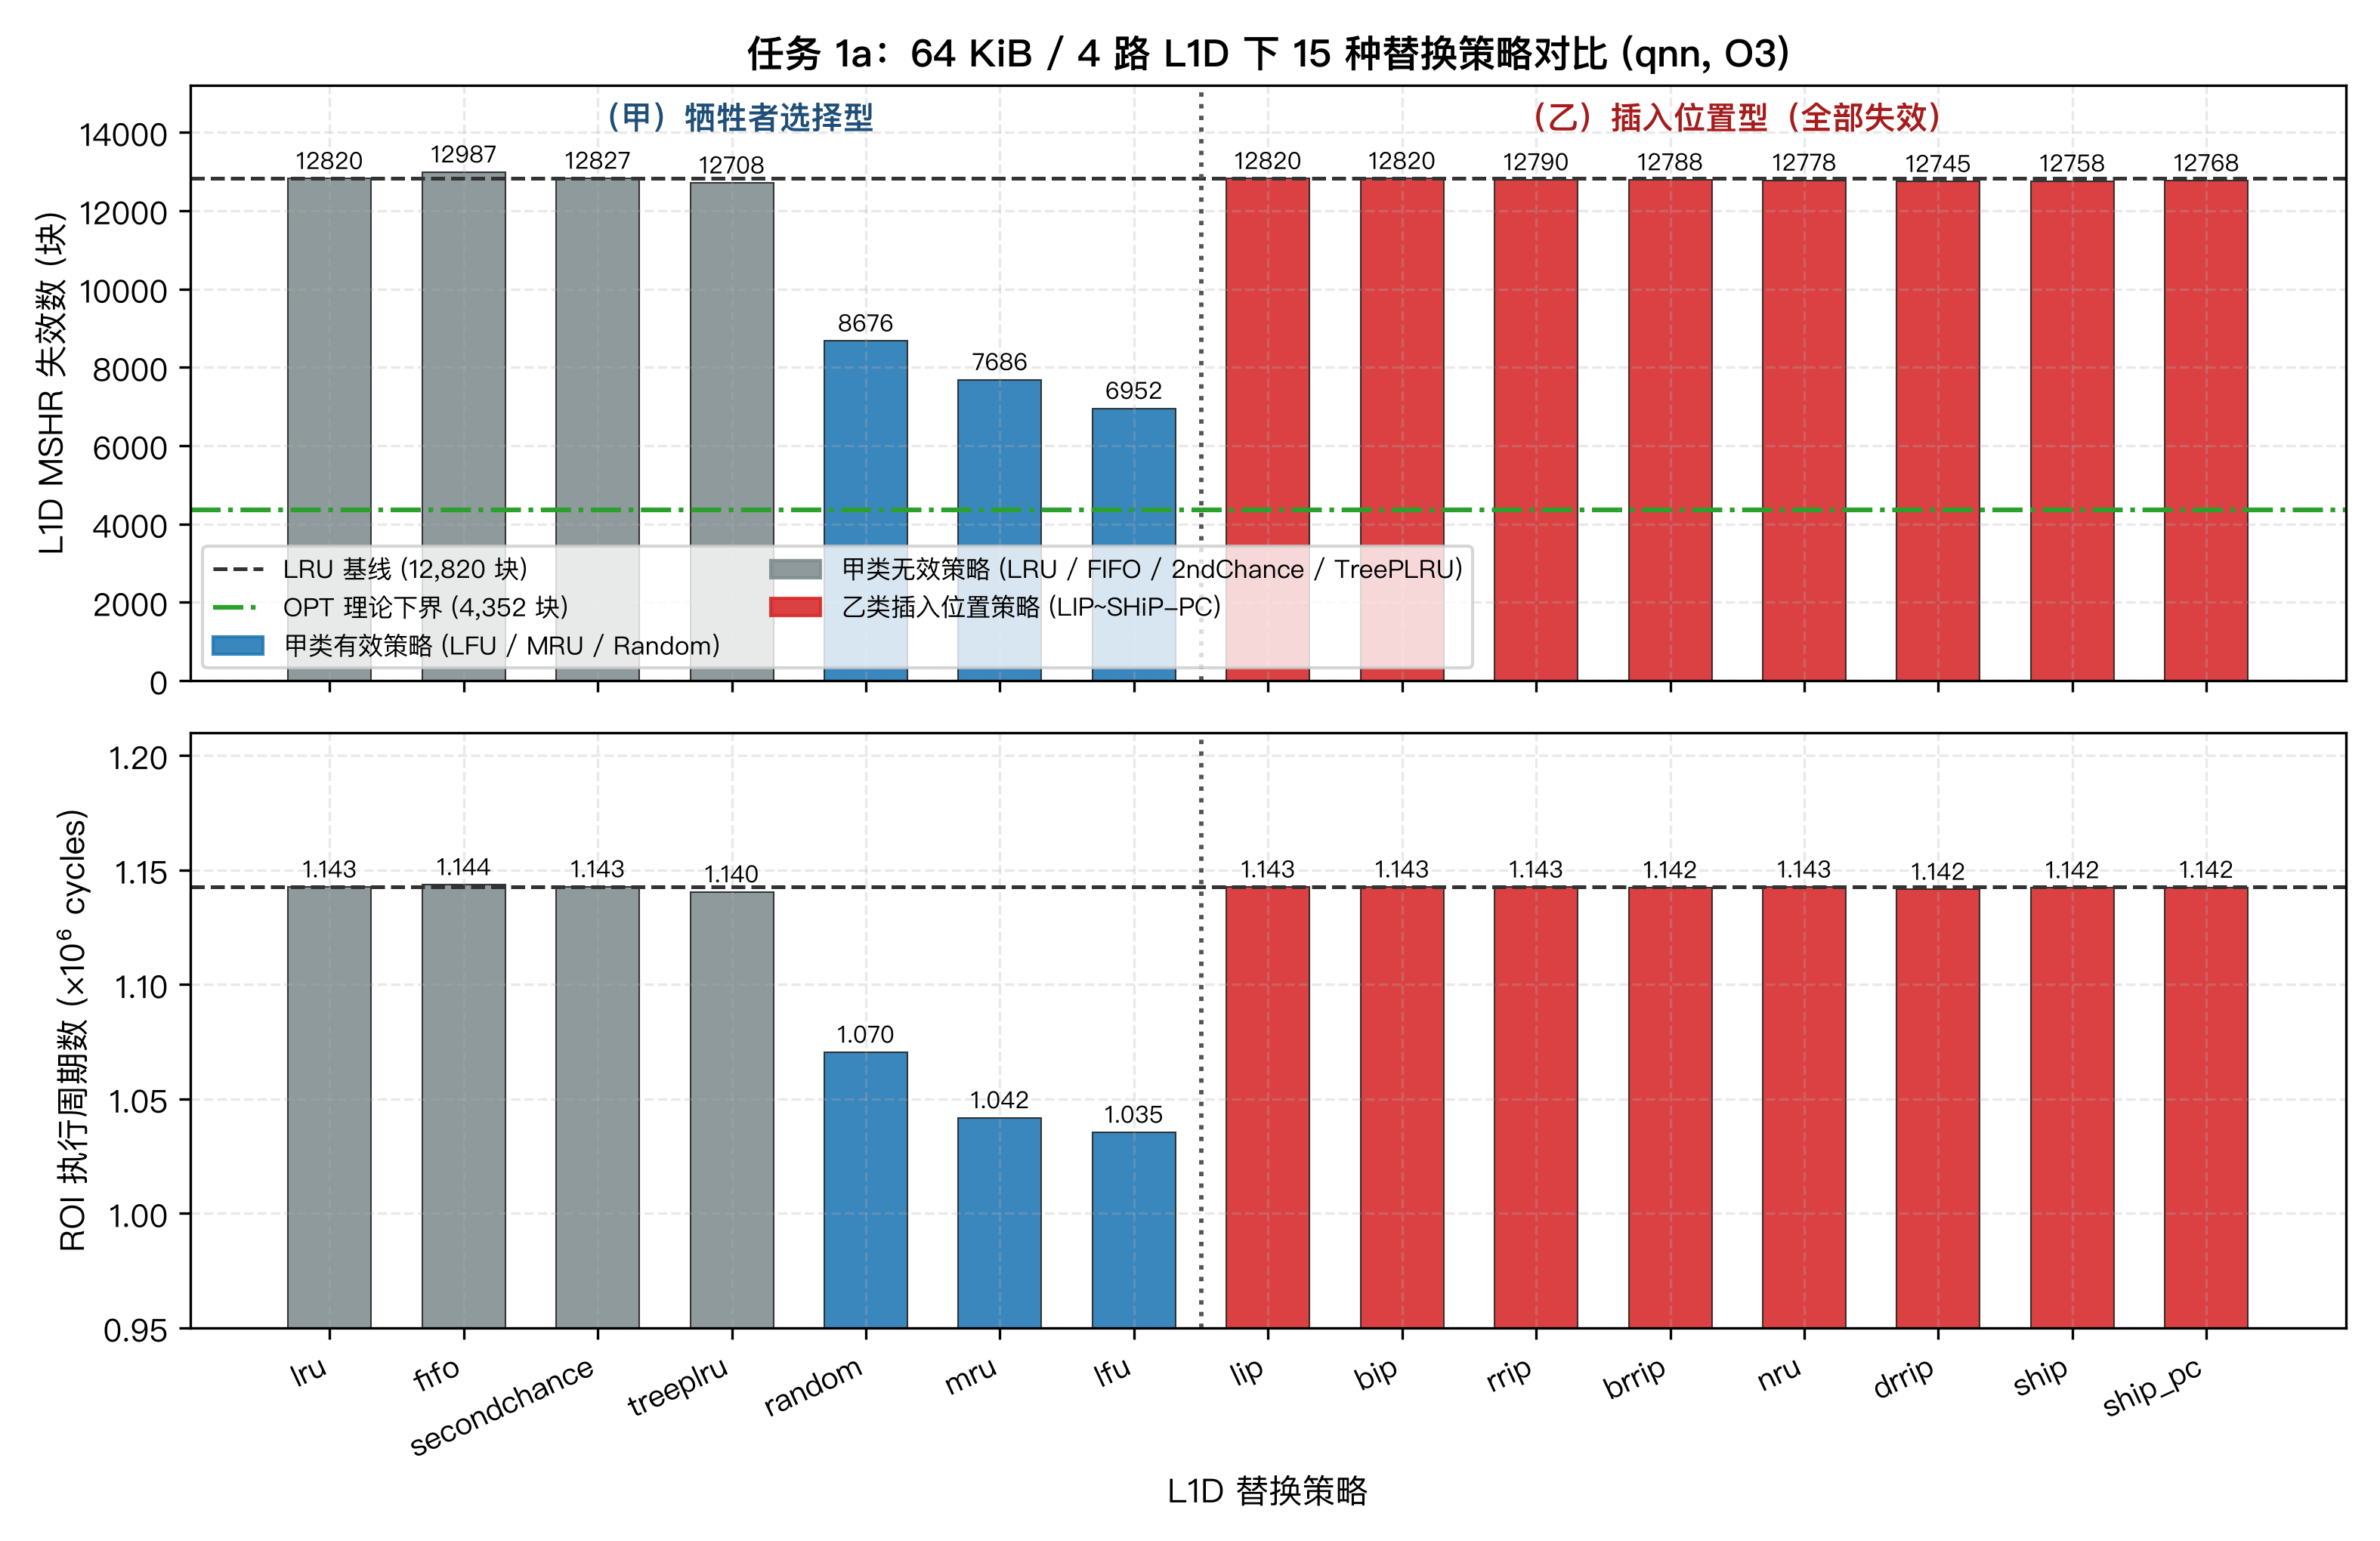
\includegraphics[width=0.96\textwidth]{fig1_l1_repl.png}
\caption{任务 1a：64 KiB / 4 路 L1D 下 15 种替换策略的 MSHR 失效数与执行周期对比}
\label{fig:l1_repl}
\end{figure}

由表~\ref{tab:t1_repl} 与图~\ref{fig:l1_repl} 可得：
\begin{enumerate}
  \item \textbf{LRU 病态验证：}\texttt{lru} 实测 \texttt{l1d\_mshr\_misses = 12\,820}（\texttt{l1d\_mshr\_mpki = 2.210}），与 $1\,568 \times 8 = 12\,544$ 仅相差 $276$ 次（$+2.20\%$），差值来自 \texttt{xbuf}、\texttt{w2}、\texttt{b1}、\texttt{hbuf} 的初始加载及少量组冲突，证实在循环扫描下 \texttt{w1} 的 L1D 复用率为精确的 0。
  \item \textbf{有效/无效划分与甲/乙分类对照：}\textbf{有效策略仅有 3 个，且全部属于（甲）牺牲者选择型}——\texttt{lfu}（$6\,952$ 次，拿下 OPT 收益的 \textbf{69.3\%}）、\texttt{mru}（$7\,686$ 次，\textbf{60.6\%}）与 \texttt{random}（$8\,676$ 次，\textbf{48.9\%}）。其余 12 个策略中，\texttt{fifo}、\texttt{secondchance} 与 \texttt{treeplru} 属于会按近似年龄全组轮换的甲类策略，无法打破循环颠簸；而\textbf{（乙）插入位置型的全部 8 个论文策略（\texttt{lip/bip/rrip/brrip/nru/drrip/ship/ship\_pc}）在 L1 上全军覆没}，失效数均停留在 $12\,745$--$12\,820$，周期与 \texttt{lru} 差异全部在 $0.09\%$ 以内（无差别）。甚至 \texttt{lip} 与 \texttt{bip} 的周期和失效数与 \texttt{lru} 逐位相等（$1\,142\,571$ 周期，$12\,820$ 次失效）。
\end{enumerate}

\subsubsection{相联度自检（任务 1b）与无病态对照组（任务 1c）}
表~\ref{tab:t1_bc} 与图~\ref{fig:assoc_nopath} 给出 64 KiB 固定容量下相联度扫描（\texttt{2/4/8/16} 路）以及消除病态的 128 KiB / 4 路对照组实测数据。

\begin{table}[H]\centering\small
\caption{任务 1b（64 KiB 相联度自检）与任务 1c（128 KiB 无病态对照组）实测结果}\label{tab:t1_bc}
\begin{tabular}{lcrrrrr}\toprule
实验组 & 相联度 & 策略 & 周期数 & 相对 LRU & IPC & \texttt{l1d\_mshr\_misses} \\\midrule
任务 1b（64 KiB） & 2 路  & \texttt{lru} & 1\,142\,571 & 基线 & 5.077 & 12\,820 \\
任务 1b（64 KiB） & 4 路  & \texttt{lru} & 1\,142\,571 & 无差别 (0.00\%) & 5.077 & 12\,820 \\
任务 1b（64 KiB） & 8 路  & \texttt{lru} & 1\,142\,571 & 无差别 (0.00\%) & 5.077 & 12\,820 \\
任务 1b（64 KiB） & 16 路 & \texttt{lru} & 1\,142\,571 & 无差别 (0.00\%) & 5.077 & 12\,820 \\
\midrule
任务 1b（64 KiB） & 2 路  & \texttt{mru} & 1\,072\,107 & $-6.17\%$ & 5.411 & 9\,230 \\
任务 1b（64 KiB） & 4 路  & \texttt{mru} & 1\,041\,769 & $-8.82\%$ & 5.568 & \textbf{7\,686} \\
任务 1b（64 KiB） & 8 路  & \texttt{mru} & \textbf{1\,041\,483} & $-8.85\%$ & \textbf{5.570} & 7\,890 \\
任务 1b（64 KiB） & 16 路 & \texttt{mru} & 1\,042\,814 & $-8.73\%$ & 5.563 & 8\,241 \\
\midrule
任务 1c（128 KiB） & 4 路 & \texttt{lru}    & \textbf{905\,805} & 基线 & \textbf{6.404} & \textbf{14} \\
任务 1c（128 KiB） & 4 路 & \texttt{bip}    & \textbf{905\,805} & 无差别 (0.00\%) & \textbf{6.404} & \textbf{14} \\
任务 1c（128 KiB） & 4 路 & \texttt{random} & 909\,863 & $+0.45\%$ & 6.375 & 126 \\
任务 1c（128 KiB） & 4 路 & \texttt{mru}    & 920\,599 & \textbf{$+1.63\%$} & 6.301 & \textbf{635} \\
\bottomrule\end{tabular}
\end{table}

\begin{figure}[H]\centering
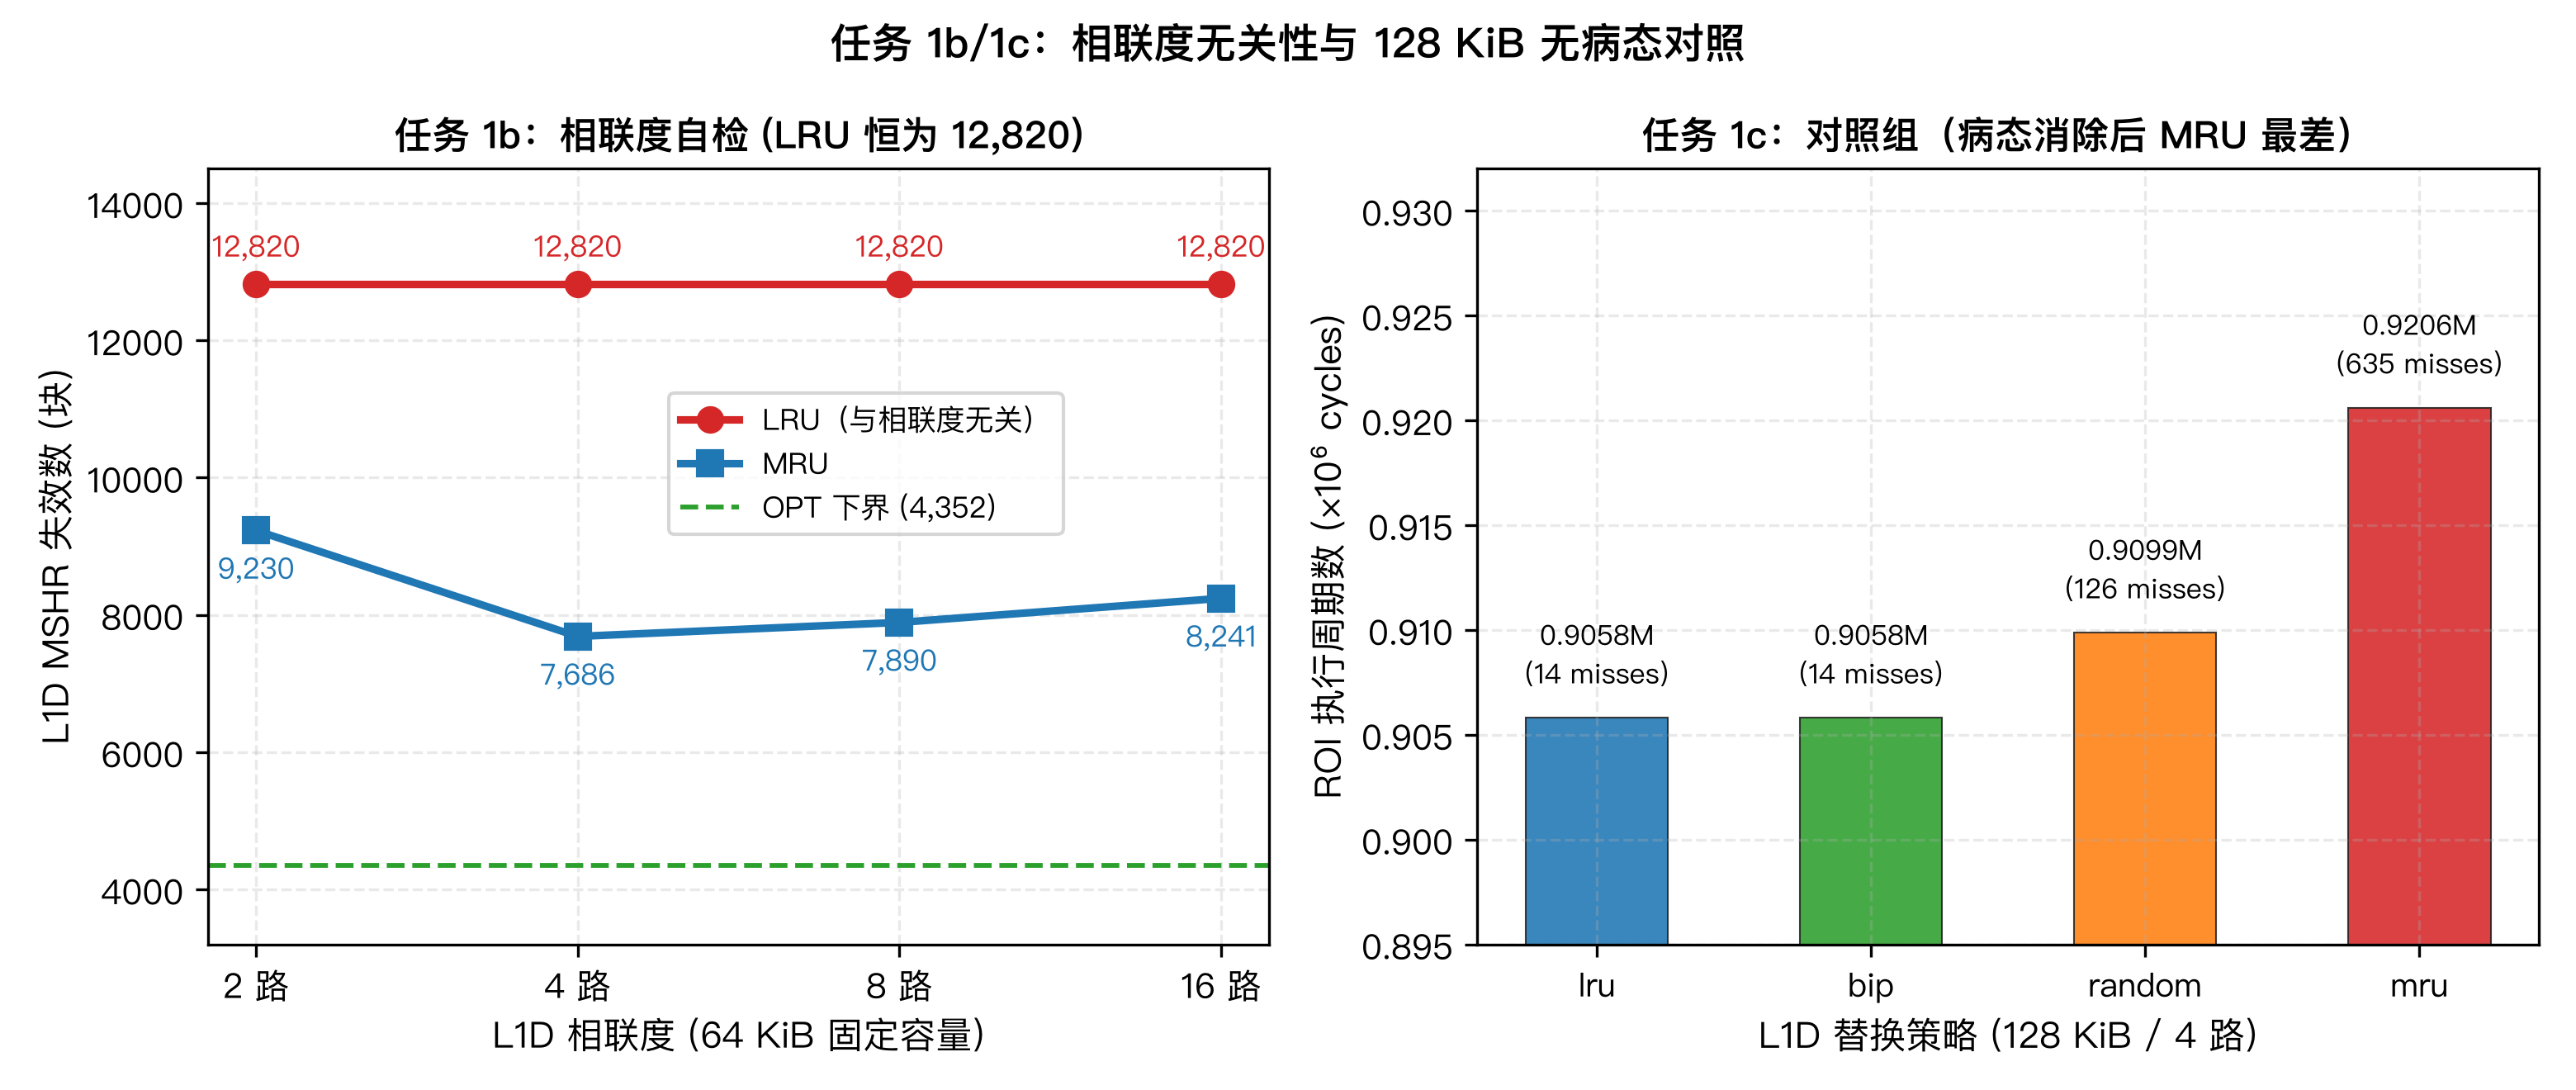
\includegraphics[width=0.96\textwidth]{fig2_assoc_nopath.png}
\caption{任务 1b 与任务 1c：相联度无关性自检与 128 KiB 无病态对照组}
\label{fig:assoc_nopath}
\end{figure}

\begin{itemize}
  \item \textbf{相联度预测检验与模型差异分析（任务 1 思考 3）：}对 \texttt{lru} 而言，相联度从 2 路升至 16 路时周期数精确锁定为 $1\,142\,571$、\texttt{l1d\_mshr\_misses} 精确锁定为 $12\,820$，完全符合 $N/A = \text{工作集}/C$ 与相联度无关的理论预测；此处不是“提高相联度能缓解”的冲突失效，而是容量不足引起的循环扫描替换失效。对于 \texttt{mru}，从 2 路升至 4 路时失效数如公式 $(A-1)/N$ 预期从 $9\,230$ 降至 $7\,686$，但升至 8 路（$7\,890$）和 16 路（$8\,241$）后反而小幅回升——原因在于简化模型假设仅存在单一扫描数组 \texttt{w1}，而固定 64 KiB 容量下相联度翻倍会使组数从 256 减半至 128 与 64 组，原本仅干扰少量组的辅助数组（\texttt{xbuf} 13 块、\texttt{w2} 20 块、\texttt{b1} 8 块等）更密集地撞入少数热组并频繁触发 \texttt{touch()}，导致 \texttt{mru} 将刚刚命中的有效驻留块或辅助块踢出（叠加 O3 乱序执行重排），即\textbf{简化单数组模型忽略了辅助数组与高相联度少组数之间的干扰}，而非测量误差。
  \item \textbf{对照组结论（任务 1c，实验诚信底线）：}当 L1D 扩至 128 KiB 后工作集完整容纳、循环扫描病态彻底消失，\texttt{lru} 与 \texttt{bip} 的失效降至仅 $14$ 次（$905\,805$ 周期），而 \texttt{random} 失效增至 $126$ 次（慢 $0.45\%$），\textbf{\texttt{mru} 失效暴增至 $635$ 次、周期数升至 $920\,599$（反比 \texttt{lru} 慢 $1.63\%$，成为四者最差）}。可见，\textbf{MRU 仅在 64 KiB 循环扫描病态下比 LRU 好；一旦病态消失，MRU 因其主动逐出刚访问块的行为反而更差}。
\end{itemize}

\subsection{任务 2：把替换策略写进 gem5}

\subsubsection{SimObject 三处注册机制（任务 2a）}
gem5 的可配置部件同时跨越 C++ 仿真内核与 Python 配置接口，新增 \texttt{CssysRP} 需协同修改 3 个框架文件外加自身 C++ 源文件。经源码树核查，\texttt{ReplacementPolicies.py}、\texttt{SConscript} 与 \texttt{framework/cssys\_se.py} 的注册 diff 如下（为保留实验一、二对未编译新内核者的兼容性，\texttt{cssys\_se.py} 使用 \texttt{try/except NameError} 挂载）：

\begin{lstlisting}[language={},caption={SimObject 三处注册的 Unified Diff（src/registration.diff）}]
--- a/gem5/src/mem/cache/replacement_policies/ReplacementPolicies.py
+++ b/gem5/src/mem/cache/replacement_policies/ReplacementPolicies.py
@@ -175,3 +175,14 @@
     type = "WeightedLRURP"
     cxx_class = "gem5::replacement_policy::WeightedLRU"
     cxx_header = "mem/cache/replacement_policies/weighted_lru_rp.hh"
+
+
+class CssysRP(BaseReplacementPolicy):
+    type = "CssysRP"
+    cxx_class = "gem5::replacement_policy::Cssys"
+    cxx_header = "mem/cache/replacement_policies/cssys_rp.hh"
+
+    evict_mru = Param.Bool(
+        False, "True: evict the most recently used way (MRU); "
+               "False: evict the least recently used way (LRU)"
+    )
--- a/gem5/src/mem/cache/replacement_policies/SConscript
+++ b/gem5/src/mem/cache/replacement_policies/SConscript
@@ -29,11 +29,12 @@
 Import('*')
 
 SimObject('ReplacementPolicies.py', sim_objects=[
-    'BaseReplacementPolicy', 'DuelingRP', 'FIFORP', 'SecondChanceRP',
+    'BaseReplacementPolicy', 'CssysRP', 'DuelingRP', 'FIFORP', 'SecondChanceRP',
     'LFURP', 'LRURP', 'BIPRP', 'MRURP', 'RandomRP', 'BRRIPRP', 'SHiPRP',
     'SHiPMemRP', 'SHiPPCRP', 'TreePLRURP', 'WeightedLRURP'])
 
 Source('bip_rp.cc')
+Source('cssys_rp.cc')
 Source('brrip_rp.cc')
--- a/framework/cssys_se.py
+++ b/framework/cssys_se.py
@@ -72,6 +72,14 @@
     "treeplru": TreePLRURP,
     "secondchance": SecondChanceRP,
 }
+
+try:
+    REPLACEMENT_POLICIES["cssys"] = CssysRP  # LRU 口径
+    REPLACEMENT_POLICIES["cssys_mru"] = lambda: CssysRP(evict_mru=True)
+except NameError:
+    pass
\end{lstlisting}

三者缺一不可：\texttt{cssys\_rp.hh/.cc} 提供 C++ 逻辑与工厂绑定；\texttt{ReplacementPolicies.py} 声明类型与参数使配置脚本可 \texttt{import}；\texttt{SConscript} 中的 \texttt{sim\_objects} 驱动构建系统生成 \texttt{params/CssysRP.hh} 与 \texttt{param\_CssysRP.cc}，\texttt{Source('cssys\_rp.cc')} 将目标文件纳入链接。

\subsubsection{阶段 2a：与 LRU 逐位相同的初始实现与验收}
首先参照 \texttt{lru\_rp.hh/.cc} 编写仅维护 \texttt{lastTouchTick}、以 \texttt{<} 选择最老时间戳的 \texttt{cssys\_rp.hh/.cc}，在 \texttt{gem5/} 下以 \texttt{scons build/RISCV/gem5.opt -j8} 编译（首次构建耗时 \texttt{2m31.83s}），随后执行 \texttt{lab3\_mine} 验收：

\begin{lstlisting}[language=bash,caption={任务 2a 逐位相同验收命令行与原始输出}]
$ python3 framework/sweep.py --name lab3_mine --bench qnn --bench-args "8 2799" \
    --base "--cpu o3 --l1d-size 64kB --l1d-assoc 4" --vary l1d-repl=lru,cssys --jobs 2
[  1/2] p000_l1d-repl-lru    ok   17.4s  ipc=5.077
[  2/2] p001_l1d-repl-cssys  ok   17.4s  ipc=5.077
$ cut -d, -f1,2,4,6,21,24,26 results/lab3_mine.csv
l1d-repl,label,cycles,ipc,l1d_misses,l1d_mshr_misses,l1d_mshr_mpki
lru,p000_l1d-repl-lru,1142571.0,5.076941,202171.0,12820.0,2.2100529481796025
cssys,p001_l1d-repl-cssys,1142571.0,5.076941,202171.0,12820.0,2.2100529481796025
\end{lstlisting}

\texttt{cssys} 与 \texttt{lru} 的 \texttt{cycles}（$1\,142\,571$）、\texttt{l1d\_misses}（$202\,171$）与 \texttt{l1d\_mshr\_misses}（$12\,820$）逐位完全一致，验证新注册的 SimObject 在模拟流水线中工作无误。

\subsubsection{阶段 2b：改一个字符的翻车、空路机制解析与修复验收}
遵循指导书 2b 步骤，先仅将 \texttt{getVictim()} 中的 \texttt{<} 改为 \texttt{>} 并增量编译（仅重编 \texttt{cssys\_rp.cc} 与 \texttt{date.cc} 并重链接，耗时 \texttt{13.55s}），运行 \texttt{lab3\_mine2\_buggy}：

\begin{lstlisting}[language=bash,caption={任务 2b 仅改一个字符时的翻车对比与修复后逐位对齐输出}]
# 仅将 '<' 改为 '>'（未处理空路 lastTouchTick == 0）
[     CXX] src/mem/cache/replacement_policies/cssys_rp.cc -> RISCV/mem/cache/replacement_policies/cssys_rp.o
[    LINK]  -> RISCV/gem5.opt   (13.551s total)
l1d-repl,label,cycles,ipc,l1d_misses,l1d_mshr_misses,l1d_mshr_mpki
mru,p000_l1d-repl-mru,1041769.0,5.568188,119251.0,7686.0,1.3249974227541672
cssys,p001_l1d-repl-cssys,1147177.0,5.056557,209174.0,13539.0,2.334002095585307

# 参照 mru_rp.cc 加入空路优先判定 (cand_data->lastTouchTick == 0) 后（13.815s total）
l1d-repl,label,cycles,ipc,l1d_misses,l1d_mshr_misses,l1d_mshr_mpki
mru,p000_l1d-repl-mru,1041769.0,5.568188,119251.0,7686.0,1.3249974227541672
cssys,p001_l1d-repl-cssys,1041769.0,5.568188,119251.0,7686.0,1.3249974227541672
\end{lstlisting}

\textbf{翻车原因剖析：}阅读 gem5 原生 \texttt{mru\_rp.cc} lines 84--92 可知，MRU 比 LRU 多了三行空路判别逻辑。系统刚上电时所有路均为空（\texttt{lastTouchTick == 0}）。首次冷失效装入 \texttt{candidates[0]} 后，\texttt{candidates[0]} 拥有非零时间戳而 \texttt{candidates[1..3]} 仍为 \texttt{0}。在 LRU 的“找最小值”循环（\texttt{<}）中，空路因 \texttt{0 < curTick()} 而天然被选中；但在单纯改为 \texttt{>} 的“找最大值”循环中，以 \texttt{victim = candidates[0]} 起步时，空路的 \texttt{0 > victim\_tick} 恒为假，导致 \texttt{candidates[1..3]} 永远无法被选作牺牲者、始终空置，4 路 Cache 退化为仅占用第 0 路的 1 路直接映射（且失效数反增至 $13\,539$）。加入 \texttt{if (cand\_data->lastTouchTick == 0) \{ victim = candidate; break; \}} 后，\texttt{cssys} 立即与 \texttt{mru} 逐位相等（$1\,041\,769$ 周期、$7\,686$ 次 MSHR 失效）。

\subsubsection{阶段 2c：参数化 \texttt{evict\_mru} 与硬件代价}
随后在 \texttt{CssysRP} 中接入 Python 参数 \texttt{evict\_mru}，在 C++ 中通过构造列表初始化成员 \texttt{const bool evictMru(p.evict\_mru)}，并将 \texttt{getVictim()} 写为 \texttt{bool better = evictMru ? (cand\_tick > victim\_tick) : (cand\_tick < victim\_tick);}，同时扩展任务 3b 统计组（完整源码见附录 A.1--A.2）。本次因头文件改动触发重编 \texttt{param\_CssysRP.cc} 与 \texttt{cssys\_rp.cc}，耗时 \texttt{17.212s}。四方联跑 \texttt{lab3\_mine3} 验收结果如下：

\begin{lstlisting}[language=bash,caption={任务 2c 参数化四方验收输出（两两逐位相等）}]
l1d-repl,label,cycles,ipc,l1d_misses,l1d_mshr_misses,l1d_mshr_mpki
lru,p000_l1d-repl-lru,1142571.0,5.076941,202171.0,12820.0,2.2100529481796025
cssys,p001_l1d-repl-cssys,1142571.0,5.076941,202171.0,12820.0,2.2100529481796025
mru,p002_l1d-repl-mru,1041769.0,5.568188,119251.0,7686.0,1.3249974227541672
cssys_mru,p003_l1d-repl-cssys_mru,1041769.0,5.568188,119251.0,7686.0,1.3249974227541672
\end{lstlisting}

可见 \texttt{lru == cssys}（$1\,142\,571$ 周期）且 \texttt{mru == cssys\_mru}（$1\,041\,769$ 周期），两两逐位相等。我们借此将一个“改源码 $+$ 重新编译”的动作转化成了“改命令行参数 $+$ 0 秒切换”的动作；在真实芯片中，这种运行时可配置能力的物理代价是：必须在控制通路增加至少一个可配置寄存器（如 CSR/模式位）来锁存 \texttt{evict\_mru}，在替换比较树/状态更新输出端增加多路选择器（MUX）与双极性比较逻辑，带来额外面积、关键路径门延迟以及软件驱动与流片前的双倍功能验证开销。

\subsection{任务 3：破案——为什么 8 个论文策略在 L1 上全军覆没}

\subsubsection{被数据否定的备选假设记录（任务 3 破案前置）}
面对 8 个插入位置型策略在 L1 上与 \texttt{lru} 差异均不到 $0.2\%$ 的反常现象，首先排查并记录以下两个被直接证伪的假设：
\begin{enumerate}
  \item \textbf{假设 0（被否定）：命令行未生效或配置脚本静默回退到 LRU。}检查 \texttt{lab3\_repl} 输出目录的 \texttt{config.ini}，实测日志如下：
  \begin{lstlisting}[language={},caption={验证 LIP 与 BRRIP 在 L1D 确实生效的 config.ini 片段}]
# out/sweeps/lab3_repl/p007_l1d-repl-lip/config.ini
replacement_policy=system.cpu.dcache.replacement_policy
response_latency=4
sequential_access=false
size=65536
--
[system.cpu.dcache.replacement_policy]
type=BIPRP
btp=0
eventq_index=0

# out/sweeps/lab3_repl/p010_l1d-repl-brrip/config.ini
[system.cpu.dcache.replacement_policy]
type=BRRIPRP
btp=3
eventq_index=0
hit_priority=false
num_bits=2
  \end{lstlisting}
  \texttt{lip} 确切实例化为 \texttt{type=BIPRP} 且 \texttt{btp=0}，\texttt{brrip} 确切实例化为 \texttt{type=BRRIPRP} 且 \texttt{btp=3, num\_bits=2}。策略在硬件配置层完全生效，假设 0 被证伪。
  \item \textbf{备选假设（被否定）：4 路组相联的槽位太少，无法容纳插入位置策略的“保留位”。}在后文任务 3c 中，将 L2 配成完全相同的 \textbf{64 KiB / 4 路} 几何结构后，同一批策略（\texttt{lip/bip/brrip/drrip/ship\_pc}）立即降低失效 $34.6\%$--$43.1\%$，证明 4 路几何本身足以支持插入位置策略生效，该假设亦被数据否定。
\end{enumerate}

\subsubsection{提出核心假设（任务 3a）}
查阅 \texttt{bip\_rp.cc} 与 \texttt{lru\_rp.cc} 源码，问题浮出水面。\texttt{LIP}（即 \texttt{btp=0} 的 \texttt{BIP}）在 \texttt{BIP::reset()} 中将新块时间戳设为 \texttt{1}（插在最老的 LRU 端）；但 \texttt{BIP} 继承自 \texttt{LRU}，其 \texttt{LRU::touch()} 在块被命中时无条件执行 \texttt{lastTouchTick = curTick()} 直接覆写。同理，\texttt{BRRIP/RRIP/DRRIP/SHiP} 在 \texttt{BRRIP::touch()} 中命中即执行 \texttt{rrpv--}（或 \texttt{rrpv.reset()} 归零）。

回到 \texttt{qnn.c} 的热点循环 \texttt{dot\_i8()}：程序按字节逐一顺序读取 64 B 的权重块。第一次访问第 0 字节触发失效并将块装入 L1D（插入“最低优先级”赌注），紧接着在极短时间内对第 1--63 字节的连续访问全部命中这同一个块！\textbf{核心假设}：在 L1D 上，丰富的\textbf{块内空间复用（intra-block hits）在插入后极短时间内就触发 \texttt{touch()}}，将原本放在最易淘汰位置的新块优先级彻底抹掉并提升至 MRU/高优先级，从而使所有插入位置型策略退化为普通 LRU。该假设给出一个可被证伪的定量预言：\textbf{在 L1D 上，每个块装入后的平均命中次数 \texttt{refsPerInsertion} 必定远大于 1，且首次命中距插入的时间 \texttt{avgFirstTouchDelay} 远小于块的平均驻留寿命}。

\subsubsection{自定义 \texttt{CssysStats} 统计量实测验证（任务 3b）}
在 \texttt{cssys\_rp.hh} 中为每块扩充元数据 \texttt{insertTick} 与 \texttt{refCount}，并定义继承自 \texttt{statistics::Group} 的 \texttt{mutable CssysStats cssysStats}。此处必须加 \texttt{mutable} 修饰：因为基类 \texttt{Base} 将 \texttt{touch()}、\texttt{reset()} 和 \texttt{getVictim()} 均声明为 \texttt{const} 成员函数，若不加 \texttt{mutable}，编译器会拒绝在这些 \texttt{const} 方法中对统计标量执行 \texttt{++} 或 \texttt{+=}（报 \texttt{cannot assign to non-static data member within const member function}）。

编译后运行 \texttt{lab3\_mine4}，提取 \texttt{stats.txt} 第二段统计块（ROI 段）中 \texttt{replacement\_policy} 相关数据：

\begin{lstlisting}[language={},caption={任务 3b：L1D（64 KiB / 4 路）ROI 段 CssysStats 实测输出}]
system.cpu.numCycles                          1142571
system.cpu.dcache.replacement_policy.insertions        12820
system.cpu.dcache.replacement_policy.touches      1439338
system.cpu.dcache.replacement_policy.victimizations        12820
system.cpu.dcache.replacement_policy.deadOnArrival            2
system.cpu.dcache.replacement_policy.victimRefSum       617283
system.cpu.dcache.replacement_policy.firstTouchDelaySum    110572001
system.cpu.dcache.replacement_policy.firstTouchCount        12820
system.cpu.dcache.replacement_policy.refsPerInsertion   112.272855
system.cpu.dcache.replacement_policy.deadFraction     0.000156
system.cpu.dcache.replacement_policy.avgFirstTouchDelay  8624.961076
\end{lstlisting}

用 2 GHz（1 周期 $= 500$ ticks）与 64 KiB 总块数（$1\,024$ 块）换算时间尺度：
\begin{align}
\text{赌注存活时间（首次命中平均延迟）} &= \frac{8\,624.961\text{ ticks}}{500\text{ ticks/cycle}} = \mathbf{17.25\text{ 周期}},\\
\text{Cache 块平均寿命} &= \frac{1\,142\,571}{12\,820 / 1\,024} = \mathbf{91\,263.1\text{ 周期}}.
\end{align}
在 L1D 上，\texttt{refsPerInsertion} 高达 \textbf{112.273}（被逐出块平均也被命中 $617\,283/12\,820 = 48.15$ 次，几乎零死块 \texttt{deadFraction} $= 0.0156\%$），新块刚装入不到 \textbf{17.25 周期}（仅占块平均寿命的 \textbf{0.019\%}）就被首次块内命中抹去了插入位置标签，假设完全成立！

\subsubsection{判决实验：64 KiB / 4 路 L2 下的策略排名反转（任务 3c）}
若假设成立，把同一批策略放到一个\textbf{看不到块内复用}的地方——L2 Cache（因为 32 KiB L1D 已在本地吸收掉全部 63 次连续字节命中），即使 L2 同样配成 64 KiB / 4 路，它们也应当立刻生效。运行 \texttt{lab3\_l2repl} 与 \texttt{lab3\_l2cssys} 后，先查看挂到 L2 上的 \texttt{CssysStats}（ROI 第二段）：

\begin{lstlisting}[language={},caption={任务 3c：L2（64 KiB / 4 路）ROI 段 CssysStats 实测输出}]
system.cpu.numCycles                          2371268
system.l2cache.overallAccesses::total           12835
system.l2cache.overallMshrMisses::total         12827
system.l2cache.replacement_policy.insertions        13367
system.l2cache.replacement_policy.touches         8311
system.l2cache.replacement_policy.victimizations        13367
system.l2cache.replacement_policy.deadOnArrival         5581
system.l2cache.replacement_policy.victimRefSum         7786
system.l2cache.replacement_policy.firstTouchDelaySum 380765265500
system.l2cache.replacement_policy.firstTouchCount         8311
system.l2cache.replacement_policy.refsPerInsertion     0.621755
system.l2cache.replacement_policy.deadFraction     0.417521
system.l2cache.replacement_policy.avgFirstTouchDelay 45814615.028276
\end{lstlisting}

表~\ref{tab:t3c_l1_l2} 将 L1（任务 1a）与 L2（任务 3c）两张表并排放（均为 64 KiB / 4 路），图~\ref{fig:l1_vs_l2} 直观展示两级 Cache 的失效降幅反转。

\begin{table}[H]\centering\scriptsize\setlength{\tabcolsep}{3.4pt}
\caption{任务 3c：相同 64 KiB / 4 路几何下 L1D 与 L2 替换策略实测并排对照（\texttt{qnn 8 2799}）}\label{tab:t3c_l1_l2}
\begin{tabular}{lrrrrrrr}\toprule
策略 & L1 周期数 & L1 失效 & L1 降幅 & L2 周期数 & \texttt{l2\_accesses} & L2 失效 & L2 降幅 \\\midrule
\texttt{lru}          & 1\,142\,571 & 12\,820 & 基线       & 2\,371\,268 & 12\,835 & 12\,827 & 基线 \\
\texttt{fifo}         & 1\,143\,589 & 12\,987 & $-1.30\%$  & 2\,364\,836 & 12\,835 & 12\,811 & $+0.12\%$ \\
\texttt{secondchance} & 1\,142\,677 & 12\,827 & $-0.05\%$  & 2\,367\,825 & 12\,835 & 12\,825 & $+0.02\%$ \\
\texttt{treeplru}     & 1\,140\,451 & 12\,708 & $+0.87\%$  & 2\,369\,626 & 12\,835 & 12\,807 & $+0.16\%$ \\
\texttt{lfu}          & \textbf{1\,035\,448} & \textbf{6\,952} & \textbf{$+45.77\%$} & 1\,944\,596 & 12\,836 & 8\,606 & $+32.91\%$ \\
\texttt{random}       & 1\,070\,414 & 8\,676  & $+32.32\%$ & 1\,926\,820 & 12\,835 & 8\,486 & $+33.84\%$ \\
\texttt{mru}          & 1\,041\,769 & 7\,686  & $+40.05\%$ & 2\,328\,198 & 12\,835 & 12\,433 & $+3.07\%$ \\
\midrule
\texttt{lip}          & 1\,142\,571 & 12\,820 & $0.00\%$   & 1\,913\,660 & 12\,836 & 8\,390 & $+34.59\%$ \\
\texttt{bip}          & 1\,142\,571 & 12\,820 & $0.00\%$   & 1\,848\,641 & 12\,836 & 7\,755 & $+39.54\%$ \\
\texttt{rrip}         & 1\,142\,523 & 12\,790 & $+0.23\%$  & 2\,367\,825 & 12\,835 & 12\,825 & $+0.02\%$ \\
\texttt{brrip}        & 1\,142\,295 & 12\,788 & $+0.25\%$  & 1\,857\,488 & 12\,836 & 7\,778 & $+39.36\%$ \\
\texttt{nru}          & 1\,142\,542 & 12\,778 & $+0.33\%$  & 2\,331\,891 & 12\,835 & 12\,457 & $+2.88\%$ \\
\texttt{drrip}        & 1\,141\,520 & 12\,745 & $+0.59\%$  & 1\,901\,203 & 12\,836 & 8\,216 & $+35.95\%$ \\
\texttt{ship}         & 1\,142\,231 & 12\,758 & $+0.48\%$  & 1\,850\,735 & 12\,835 & 7\,823 & $+39.01\%$ \\
\texttt{ship\_pc}     & 1\,142\,408 & 12\,768 & $+0.41\%$  & \textbf{1\,801\,789} & 12\,836 & \textbf{7\,301} & \textbf{$+43.08\%$} \\
\bottomrule\end{tabular}
\end{table}

\begin{figure}[H]\centering
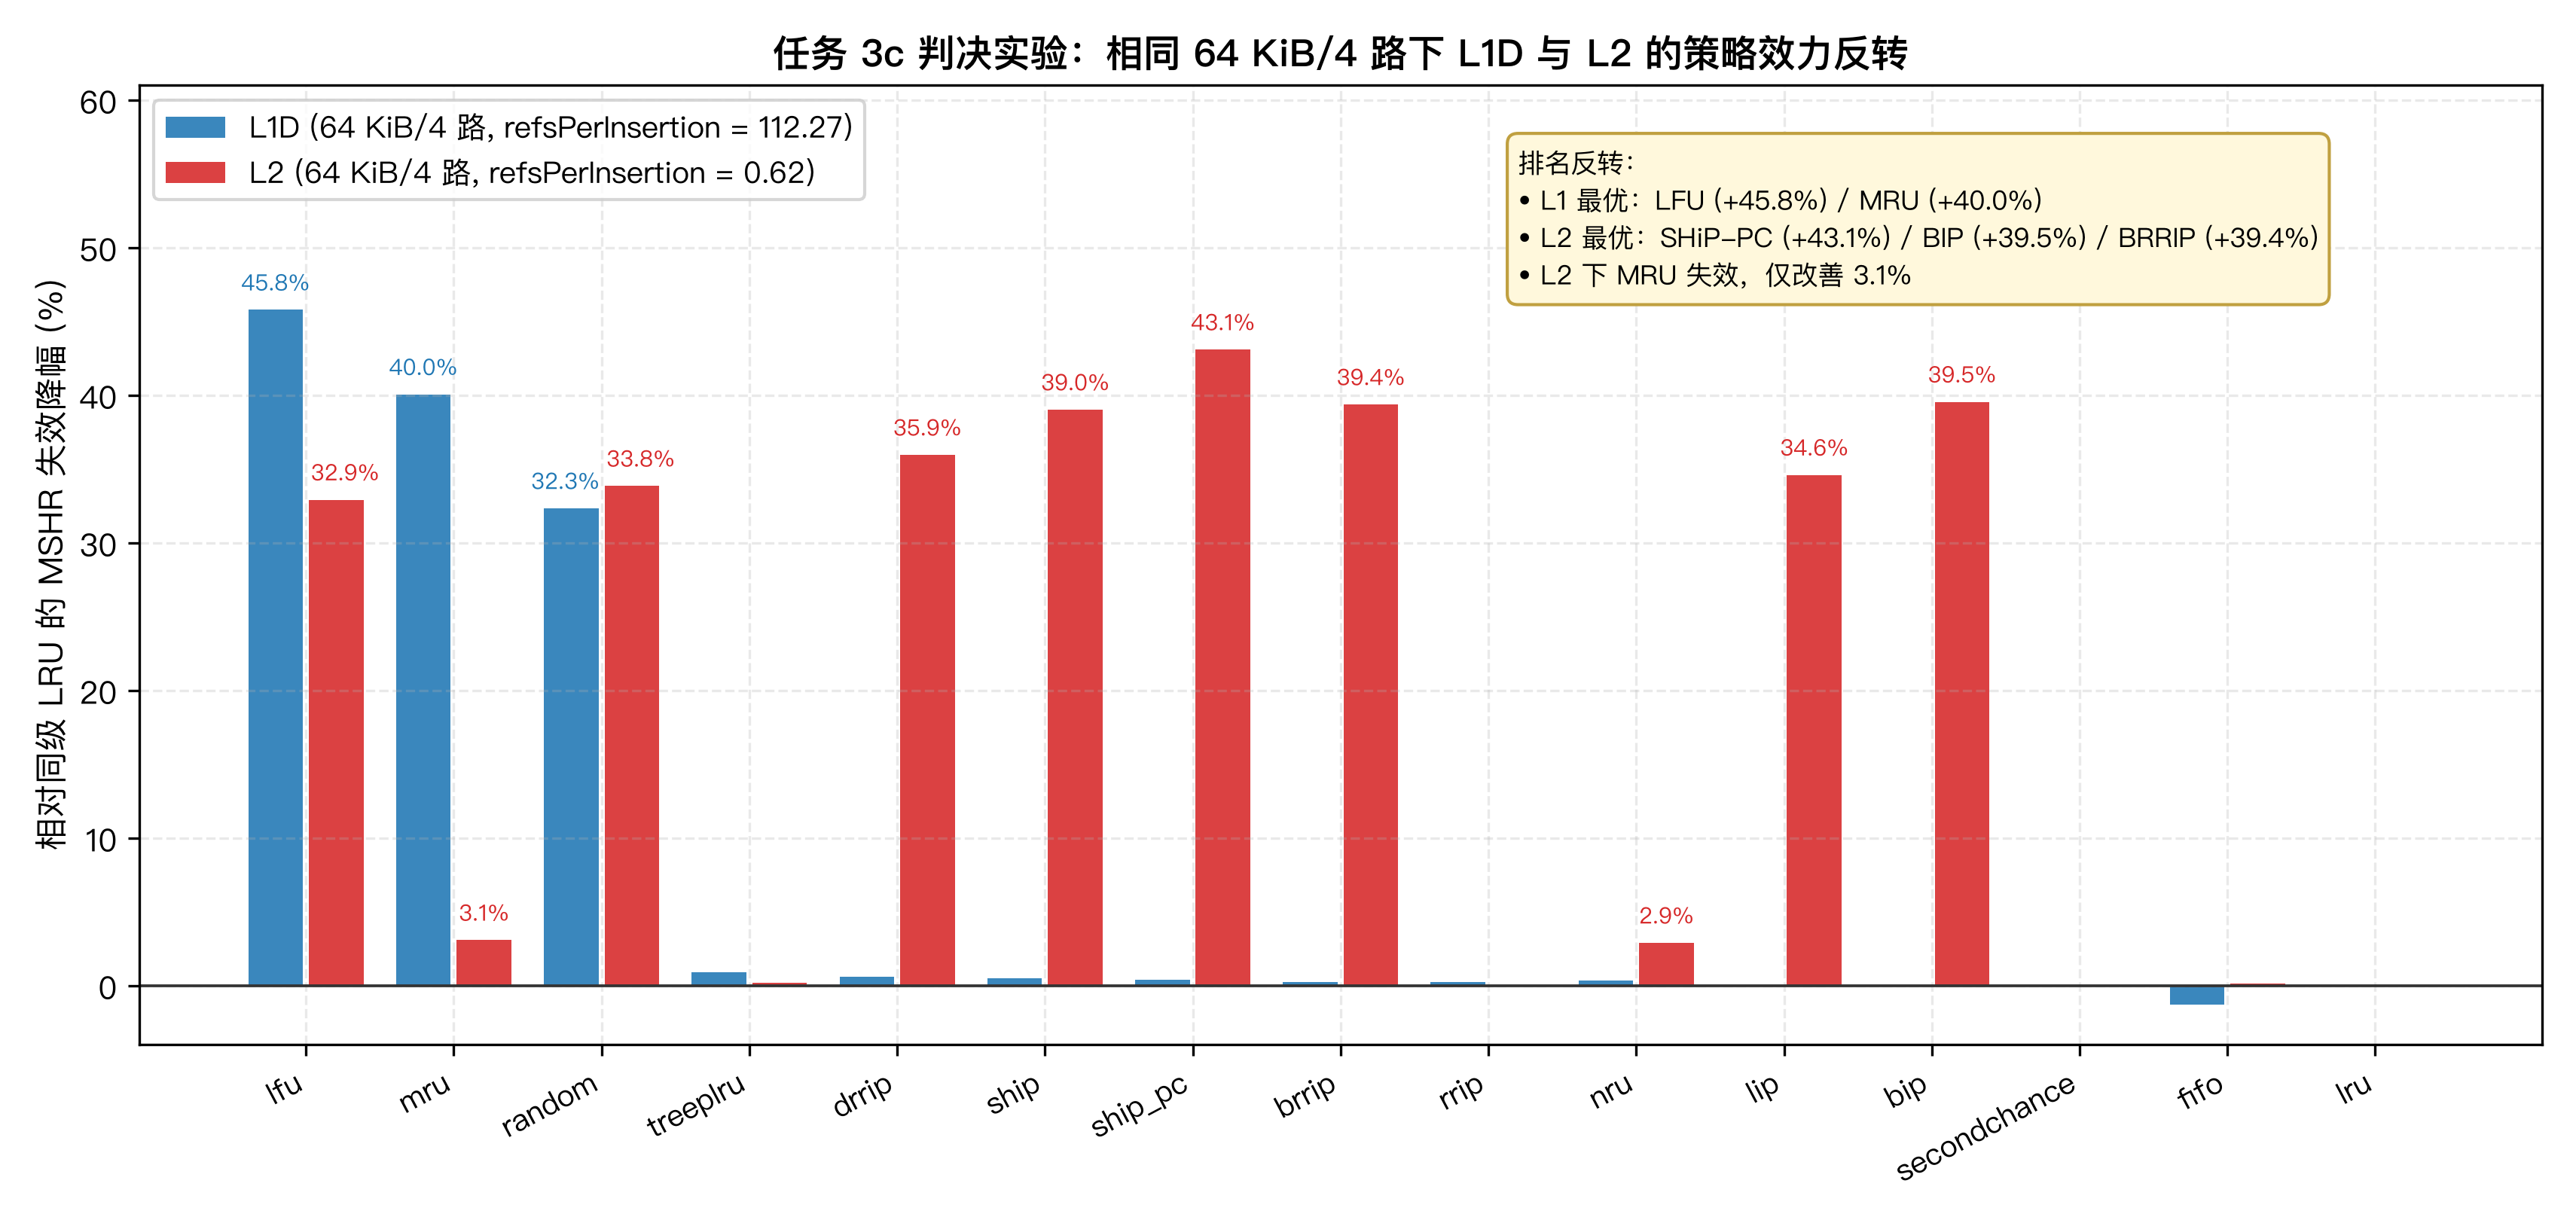
\includegraphics[width=0.98\textwidth]{fig3_l1_vs_l2_inversion.png}
\caption{任务 3c 判决实验：相同 64 KiB / 4 路几何下 L1D 与 L2 的策略降幅反转}
\label{fig:l1_vs_l2}
\end{figure}

基于表~\ref{tab:t3c_l1_l2}、图~\ref{fig:l1_vs_l2} 与 gem5 源码，逐一回答任务 3c 的全部 5 个问题（含两道加分题）：
\begin{enumerate}
  \item \textbf{最优策略反转：}在同一程序、同一 98 KiB 工作集、完全一致的 64 KiB / 4 路几何下，\textbf{L1D 上最优的是 \texttt{lfu}（$6\,952$ 次失效，降幅 $45.77\%$）与 \texttt{mru}（$7\,686$ 次，降幅 $40.05\%$）}，8 个插入位置型策略全数无效；而在 \textbf{L2 上最优的是 \texttt{ship\_pc}（$7\,301$ 次，降幅 $43.08\%$，周期降 $24.02\%$）}，紧随其后的是 \texttt{bip}（$+39.54\%$）、\texttt{brrip}（$+39.36\%$）、\texttt{ship}（$+39.01\%$）、\texttt{drrip}（$+35.95\%$）与 \texttt{lip}（$+34.59\%$），几乎完美包揽前排。
  \item \textbf{用 \texttt{refsPerInsertion} 解释反转：}L1D 的 \texttt{refsPerInsertion} 高达 \textbf{112.273}（首次触达仅 $17.25$ 周期），而 L2 骤降至 \textbf{0.622}（差近 180 倍！且在 L2 上首次触达延迟升至 $45\,814\,615\text{ ticks} = \mathbf{91\,629}$ 周期，占块平均寿命 $181\,655$ 周期的一半，\texttt{deadFraction} 高达 $41.75\%$）。这是因为 L1D 已在核侧吸收了全部 63 次块内字节访问，到达 L2 的是粗粒度行流——块被装入 L2 后不会立刻迎来第二次访问，插入位置策略下的“冷插入赌注”得以安然存活整整一轮扫描周期，使大部分扫描流在被再次访问前就被原地淘汰，从而保住高价值常驻块。
  \item \textbf{为什么 \texttt{mru} 在 L1 排前三、在 L2 却几乎没用（仅改善 3.07\%）：}查阅 \texttt{mru\_rp.cc} 可知，\texttt{MRU::touch()} 将刚命中的块时间戳更新为 \texttt{curTick()}，而 \texttt{MRU::getVictim()} 专门淘汰\texttt{lastTouchTick} \textbf{最大}（刚刚命中）的块。在 L1 上，一个块刚被装入时会立刻经历约 63 次连续命中，命中期间每轮组内都会选到它并将其踢出——从而把其余 $A-1$ 块永远钉在 Cache 里；而在 L2 上不仅单块在一个样本周期内极少迎来需求命中（L2 \texttt{overallHits = 8}），更深层的原因可通过核查 \texttt{gem5/src/mem/cache/base.cc:1256} 解释：\texttt{BaseCache::access()} 对一切入站报文先执行 \texttt{tags->accessBlock(pkt)} 并调用 \texttt{replacementPolicy->touch()}。L1D（32 KiB，\texttt{writeback\_clean=false}）在逐出干净块时会向 L2 发送 \texttt{CleanEvict}（另加 \texttt{WritebackDirty}），这些报文恰好约在块装入 L2 很久之后到达，一旦命中 L2 中的常驻块就触发了 $8\,311$ 次 \texttt{touch()}（在 \texttt{mru} 上把好不容易留存下来的块立刻标记为“最新访问 $= $ 下一顺位牺牲品”并随后逐出，使 \texttt{mru} 的 L2 需求命中仅 402 次、远逊于 \texttt{lip} 的 $4\,446$ 次与 \texttt{bip} 的 $5\,081$ 次）。
  \item \textbf{加分题（\texttt{lfu} vs \texttt{lip}）：}查阅 \texttt{lfu\_rp.cc}（lines 55--84）与 \texttt{lru\_rp.cc}（lines 57--88）：\texttt{LFU::reset()} 与 \texttt{LIP} 的 \texttt{BIP::reset()} 一样都将新块放在最低优先级（\texttt{refCount = 1} 对 \texttt{lastTouchTick = 1}），但两者的 \texttt{touch()} 本质不同——\textbf{\texttt{LRU::touch()} 执行的是“覆写”（\texttt{lastTouchTick = curTick()}），单次命中即擦除全部历史差异并使新块一跃成为最新块；而 \texttt{LFU::touch()} 执行的是“累加”（\texttt{refCount++}）}。在 L1 上，前几轮得以幸存的老块在跨样本循环中持续累加 \texttt{refCount}（升至 $100+$、$200+$），新进入并仅靠一次扫描获得约 48--64 次块内命中的块，其计数始终严格小于老块，无法将已钉住的老块挤出，从而稳定保住约半数工作集（\texttt{lfu} 在 L1 上取得 45.77\% 的全场最高降幅，在 L2 上也保住 32.91\% 的降幅）。
  \item \textbf{加分题（\texttt{rrip} vs \texttt{brrip}）：}阅读 \texttt{brrip\_rp.cc}（lines 77--92）与 \texttt{ReplacementPolicies.py}（lines 105--120）可知，\texttt{RRIPRP} 与 \texttt{BRRIPRP} 在 gem5 中同属 \texttt{BRRIP} 类（默认 \texttt{num\_bits = 2}，最大 \texttt{RRPV = 3}），唯一区别在于参数 \texttt{btp}：
  \begin{lstlisting}[language=C++,caption={gem5 brrip\_rp.cc 中 RRPV 插入逻辑}]
casted_replacement_data->rrpv.saturate();      // 先置为最大值 2^2-1 = 3 (distant)
if (rng->random<unsigned>(1, 100) <= btp) {
    casted_replacement_data->rrpv--;           // 概率<=btp 时减1变成 2 (long)
}
  \end{lstlisting}
  \texttt{rrip} 设 \texttt{btp=100}（即纯 SRRIP），\textbf{100\% 的新块全部插在 \texttt{RRPV=2}}（较长重用间隔）。在 L2 上无块内命中，整组很快全部填满 \texttt{RRPV=2} 的块；当需要淘汰时，\texttt{getVictim()} 因找不到 \texttt{RRPV=3} 而计算 \texttt{diff = 3 - 2 = 1}，将同组所有块统一老化至 \texttt{3} 后淘汰最早插入者，完全退化为同步老化颠簸（失效 $12\,825$ 次，与 \texttt{lru} 无差别）。而 \texttt{brrip} 设 \texttt{btp=3}，\textbf{将 97\% 的新块直接插在 \texttt{RRPV=3}（最远距离、即插即踢）}，仅有 3\% 概率插在 \texttt{RRPV=2}；这样既不会因 \texttt{diff} 老化掉已留驻的 \texttt{RRPV=2/1/0} 热块，又让少数幸存块在下一轮命中后降至 \texttt{RRPV=1/0} 牢牢钉在 L2 中，因此 \texttt{brrip} 在 L2 上立刻带来 \textbf{39.36\% 的失效下降（周期加速 27.7\%）}。
\end{enumerate}

\subsection{任务 4：硬件预取器的收益、代价与方法学陷阱}
回到实验二默认基线（32 KiB / 2 路 L1D，64 B 块），固定容量仅扫描 5 种预取器，实测数据见表~\ref{tab:t4_pf} 与图~\ref{fig:prefetchers}。

\begin{table}[H]\centering\footnotesize\setlength{\tabcolsep}{4pt}
\caption{任务 4：32 KiB / 2 路 L1D 下五种硬件预取器实测对比（\texttt{qnn 8 2799}）}\label{tab:t4_pf}
\begin{tabular}{lrrrrrrrrr}\toprule
预取器 & 周期数 & IPC & \texttt{l1d\_misses} & \texttt{mshr\_mpki} & 发出数 & 有用数 & 准确率 & 覆盖率 & \texttt{l1d\_mlp} \\\midrule
\texttt{none}   & 1\,102\,090 & 5.263 & 202\,290 & 2.211 & 0 & 0 & 0.00\% & 0.00\% & 15.769 \\
\texttt{tagged} & \textbf{890\,858} & \textbf{6.511} & \textbf{3\,492} & 2.221 & 25\,257 & 12\,569 & 49.76\% & \textbf{98.00\%} & 0.271 \\
\texttt{stride} & 891\,035 & 6.510 & 3\,613 & 2.227 & 49\,137 & 12\,566 & 25.57\% & 97.96\% & 0.280 \\
\texttt{bop}    & 913\,451 & 6.350 & 23\,676 & 2.223 & 11\,356 & 11\,286 & \textbf{99.38\%} & 87.98\% & 1.836 \\
\texttt{ampm}   & 891\,042 & 6.510 & 3\,637 & 2.259 & 170\,753 & 12\,560 & 7.36\% & 97.96\% & 0.278 \\
\texttt{isb}    & 1\,102\,090 & 5.263 & 202\,290 & 2.211 & 114 & 0 & 0.00\% & 0.00\% & 15.769 \\
\bottomrule\end{tabular}
\end{table}

\begin{figure}[H]\centering
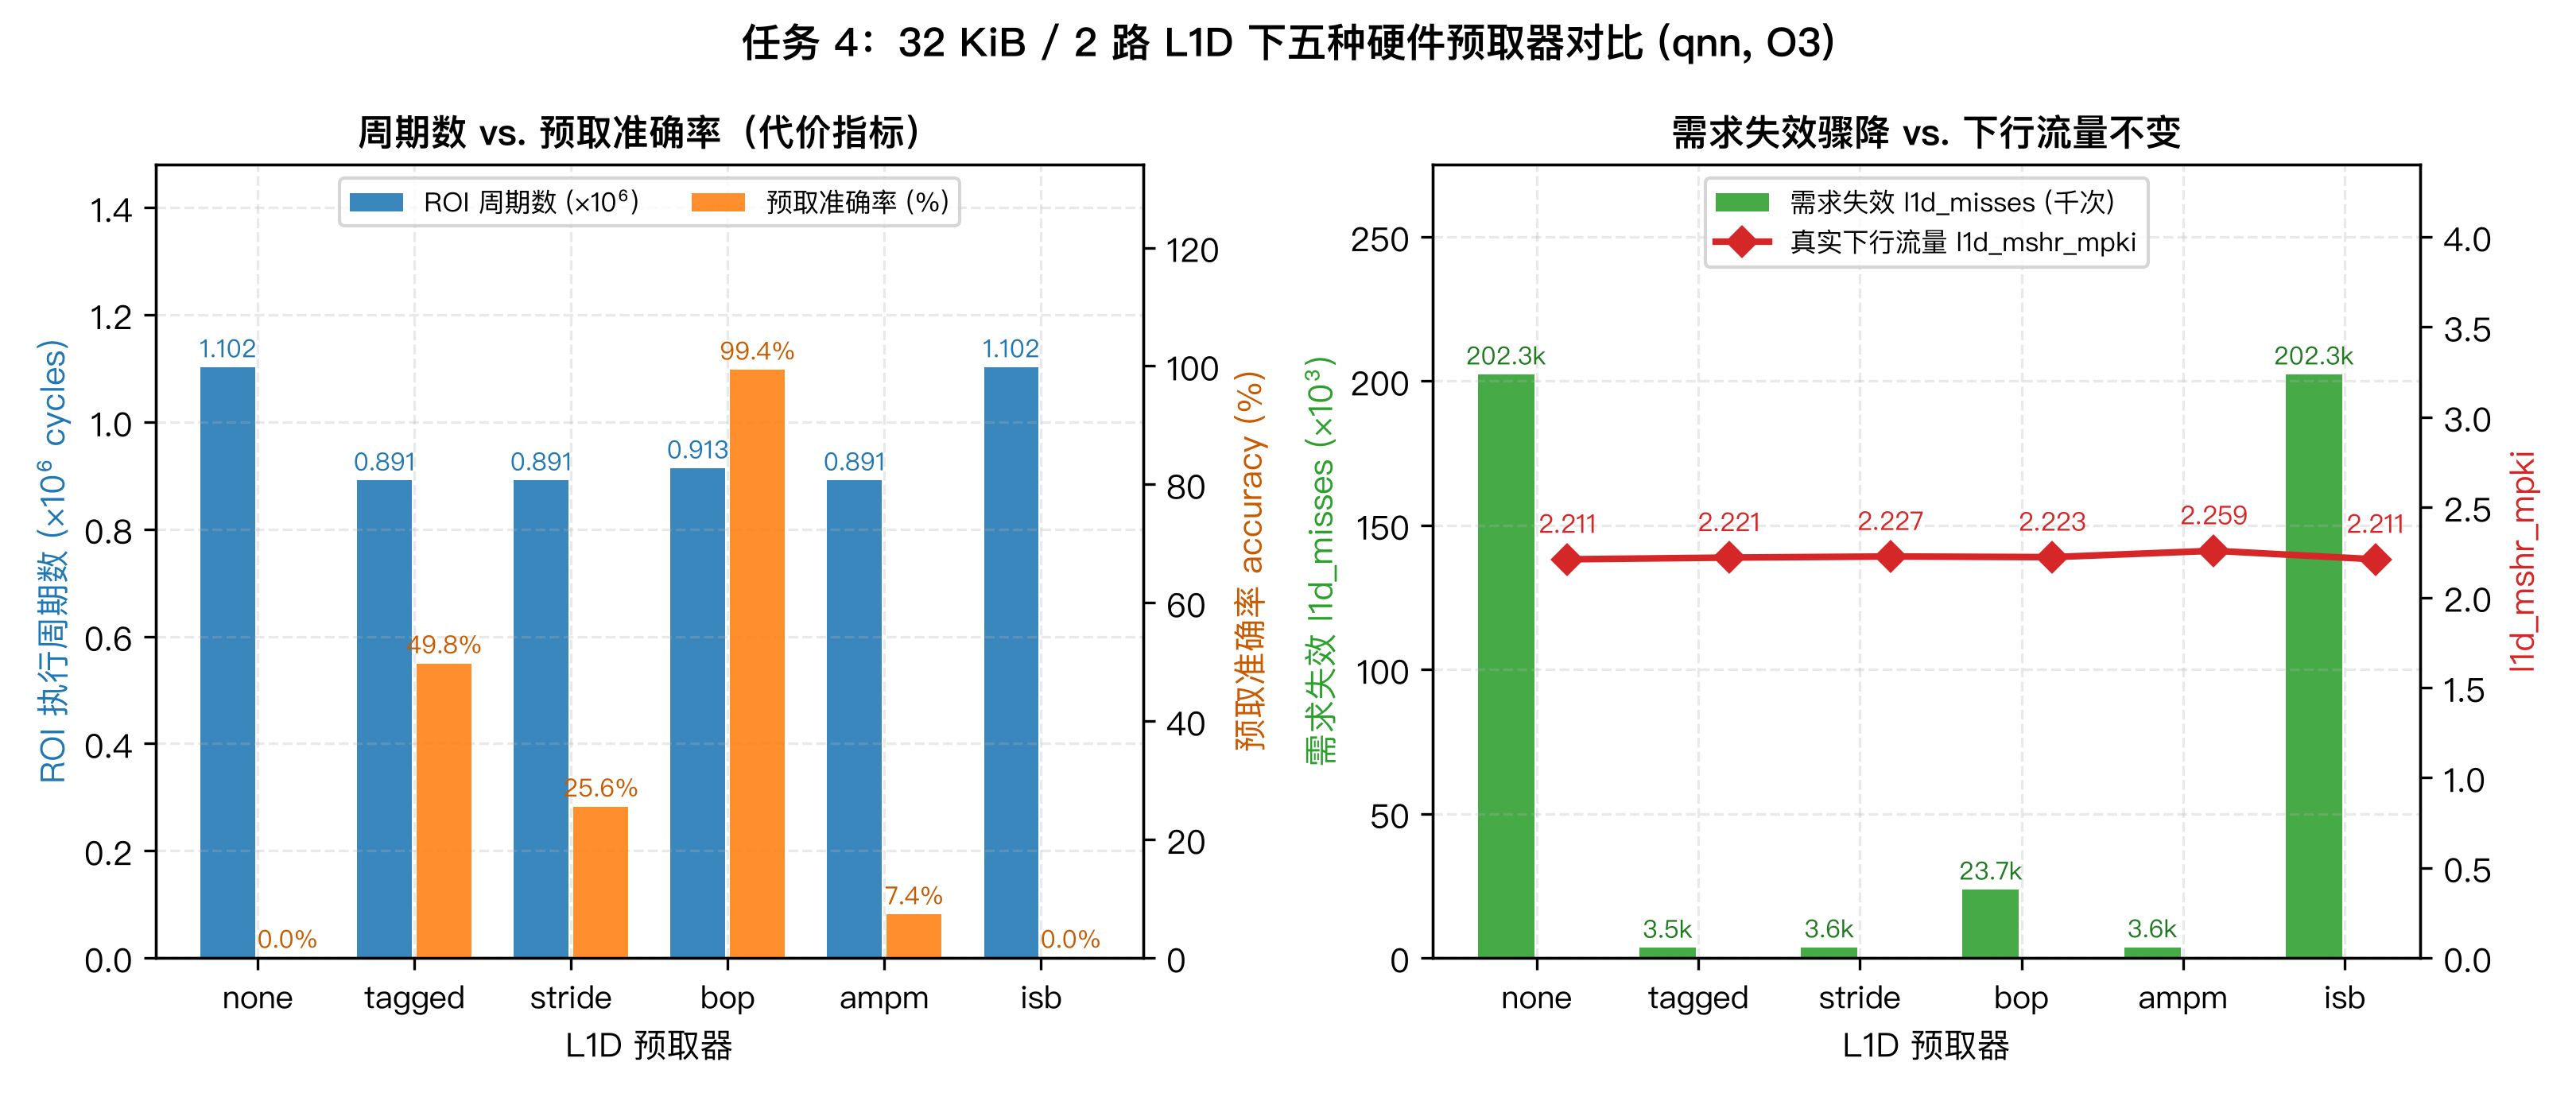
\includegraphics[width=0.98\textwidth]{fig4_prefetchers.png}
\caption{任务 4：32 KiB / 2 路 L1D 下五种硬件预取器的性能、准确率与下行流量对比}
\label{fig:prefetchers}
\end{figure}

\begin{enumerate}
  \item \textbf{准确率是代价指标而非收益指标（问题 1）：}\texttt{tagged}（$890\,858$ 周期）、\texttt{stride}（$891\,035$ 周期）与 \texttt{ampm}（$891\,042$ 周期）三者执行周期几乎完全相等（差异 $<0.021\%$，无差别），但它们的预取准确率却相差近 7 倍（分别为 \textbf{49.76\%}、\textbf{25.57\%}、\textbf{7.36\%}）；而 \texttt{bop} 准确率高达 \textbf{99.38\%}（相差十余倍），却因覆盖率较低（87.98\% vs 98.0\%）导致周期数反慢于三者（$913\,451$ 周期）。决定性能的是有用预取数量（\texttt{pfUseful} $\approx 12\,560$）和覆盖率；而发出的多余无用预取（\texttt{ampm} 发出 $170\,753$ 次，其中 $15.8$ 万次冗余或已在 Cache 命中被过滤）直接体现在低准确率和额外控制/查询功耗上，证明\textbf{准确率是衡量带宽与能耗浪费的代价指标，覆盖率才是收益指标}。
  \item \textbf{需求失效骤降而真实流量不变（问题 2）：}开启 \texttt{tagged/stride/ampm} 后，\texttt{l1d\_misses} 从 $202\,290$ 暴跌至 $3\,492$--$3\,637$（降幅 98.2\%），但真实下行流量 \texttt{l1d\_mshr\_mpki} 却维持在 $2.221$--$2.259$（相对基线 $2.211$ 基本不变）。依据 §1.8 机制，\textbf{预取不增加 Cache 有效容量，无法把块留在 L1D 里，8 遍扫描所需的 98 KiB 权重流量依然得一遍不落地从 L2 搬进来}——只不过原本由 CPU 需求加载（\texttt{ReadSharedReq}）产生的失效，提前变成了由硬件预取（\texttt{HardPFReq}）发往 L2 的请求，数据抵达时间提前、总搬运字节数守恒。
  \item \textbf{为什么 \texttt{isb} 在 \texttt{qnn} 上发了 114 次预取却一次没用上（问题 3）：}查阅 \path{gem5/src/mem/cache/prefetch/irregular_stream_buffer.cc} 可知，ISB（Irregular Stream Buffer）是为链表/指针追逐等不规则地址相关性设计的时序流预测器：它用 PC 索引 \texttt{TrainingUnit} 配对前后物理块地址 $(A, B)$ 并分配结构地址 $S$ 写入 PS-AMC/SP-AMC（默认各仅 128 项），且仅在默认 \texttt{on\_miss} 路径下学习、当精确映射置信度达到阈值才发预取。在 \texttt{qnn} 上，\texttt{dot\_i8()} 拥有稳定线性 $+64\text{ B}$ 步长、高达 $1\,568$ 个不同权重块远超 128 项 AMC 容量，加上 O3 并行乱序请求使同一 PC 的相邻缺失地址跳变、新建立的结构流映射在下一轮回到同一地址前早已因容量置换而被冲刷，最终仅在局部边界误触发 114 次（全部 \texttt{pfLate} 且 \texttt{pfUseful = 0}）。
  \item \textbf{方法学陷阱——为什么开预取后 \texttt{l1d\_mlp} 变成 $0.27$（问题 4）：}查验 \path{framework/stats.py:122} 与 \path{gem5/src/mem/cache/base.cc} 的计数定义，并读取 \texttt{stride} 实测 ROI 原始计数器：
  \begin{lstlisting}[language={},caption={任务 4 方法学陷阱：framework/stats.py 与 gem5/base.cc 口径及 stride 实测计数}]
# framework/stats.py:122
row[f"{level}_mlp"] = (miss / mshr_miss) if mshr_miss else 0.0
# 即 overallMisses::total / overallMshrMisses::total

# out/sweeps/lab3_pf/p002_l1d-pf-stride/stats.txt (ROI 第二段)
system.cpu.dcache.demandMisses::total               3613
system.cpu.dcache.overallMisses::total              3613
system.cpu.dcache.demandMshrMisses::total            262
system.cpu.dcache.HardPFReq.mshrMisses::total      12657
system.cpu.dcache.overallMshrMisses::total         12919  # = 262 + 12657
  \end{lstlisting}
  在 gem5 的 \texttt{base.cc:2344} 与 \texttt{2454} 中，\texttt{overallMisses} 与 \texttt{overallMshrMisses} 理论上都包含需求（demand）与非需求（\texttt{HardPFReq}）两部分；但硬预取请求是在 \texttt{Cache::getNextPacket()}（\texttt{base.cc:936}）中直接通过 \texttt{mshrMisses++} 分配 MSHR 发出的，\textbf{从未走过需求访问路径，因此根本不累加 \texttt{HardPFReq.misses}}！结果分子 \texttt{overallMisses} 仅剩需求失效 $3\,613$，而分母 \texttt{overallMshrMisses} 却同时计入了需求 MSHR 失效（$262$）和硬件预取 MSHR 失效（$12\,657$），于是计算得出 $3\,613 / 12\,919 = 0.280 < 1$（而真实需求 MLP 为 \texttt{demandMisses / demandMshrMisses} $= 3\,613 / 262 = 13.79$）。因此，\textbf{\texttt{overallMisses/overallMshrMisses} 作为 MLP 度量的隐含前提是“不存在由预取器绕过 \texttt{access()} 直接插入 MSHR 的流量”（即关闭硬件预取）}，一旦开启预取器该口径即超出了适用范围。
\end{enumerate}

\subsection{任务 5：预取 vs. 加容量与最终配置提案重写（核心交付物）}
表~\ref{tab:t5_cmp} 与图~\ref{fig:pf_vs_size_pchase}（左栏）汇总了不同 L1D 容量搭配 \texttt{none/stride} 的性能、流量及 \path{framework/area.py} 评估结果。

\begin{table}[H]\centering\footnotesize\setlength{\tabcolsep}{3.8pt}
\caption{任务 5：L1D 容量与 Stride 预取器对比及面积/能量评估（\texttt{qnn 8 2799}）}\label{tab:t5_cmp}
\begin{tabular}{llrrrrrrrr}\toprule
L1D 容量 & 预取器 & 周期数 & IPC & \texttt{mshr\_mpki} & L1D 面积($A$) & 总面积($A$) & 总能量($E$) & \texttt{ADP} \\\midrule
32 KiB  & \texttt{none}   & 1\,102\,090 & 5.263 & 2.2114 & 43.2  & 836.0 & 43\,337\,532 & 921.38 \\
\textbf{32 KiB} & \textbf{\texttt{stride}} & \textbf{891\,035} & \textbf{6.510} & 2.2271 & \textbf{47.2} & \textbf{840.0} & \textbf{36\,883\,411} & \textbf{748.50} \\
64 KiB  & \texttt{none}   & 1\,142\,571 & 5.077 & 2.2101 & 80.4  & 873.2 & 48\,767\,082 & 997.71 \\
64 KiB  & \texttt{stride} & 895\,265    & 6.479 & 2.2149 & 84.4  & 877.2 & 41\,125\,775 & 785.34 \\
128 KiB & \texttt{none}   & 905\,805    & 6.404 & \textbf{0.0024} & 154.7 & 947.6 & 47\,197\,289 & 858.32 \\
128 KiB & \texttt{stride} & 905\,590    & 6.406 & 0.0017 & 158.7 & 951.6 & 47\,219\,314 & 861.74 \\
\bottomrule\end{tabular}
\end{table}

\begin{enumerate}
  \item \textbf{\texttt{32kB + stride} vs \texttt{128kB + none} 的性能与面积对比（问题 1）：}\texttt{32kB + stride} 仅用 $891\,035$ 周期，甚至比 \texttt{128kB + none}（$905\,805$ 周期）还快 \textbf{1.63\%}（因为 32 KiB 的命中延迟仅为 3 周期，而 128 KiB 高达 5 周期，预取器成功掩盖了 L2 访问延迟后 32 KiB 享受到低命中延迟红利）。面积上直接省下 96 KiB 数据 SRAM 及其配套 Tag/Mux 开销：依据 \texttt{area.py} 模型，L1D 面积从 $154.7\ A$ 暴降至 $47.2\ A$（\textbf{仅 L1D 节省 69.5\%}，芯片总面积从 $947.6\ A$ 降至 $840.0\ A$ 节省 11.4\%），总能量因单次访问小容量 SRAM 更省电且执行时间更短而降低 \textbf{21.85\%}（ADP 改善 12.8\%）。
  \item \textbf{下行流量差距与多核共享 L2 场景下的风险（问题 2）：}\texttt{32kB + stride} 的 \texttt{l1d\_mshr\_mpki} 为 \textbf{2.2271}，而 \texttt{128kB + none} 仅为 \textbf{0.0024}——两者相差逾 \textbf{920 倍}（L2 访问数 $12\,927$ vs $14$）！这直接证明两者物理机制截然不同：\texttt{128kB} 把数据留在 L1D 里从而彻底消灭了总线流量，而 \texttt{stride} 只是把 L2 流量提前发送。在\textbf{多核共享 L2 的场景下，\texttt{32kB + stride} 会明显更糟}：多个核每轮持续向共享 L2 倾泻大量预取流量（且 \texttt{stride} 准确率仅 25.6\%，虽然一部分被过滤，仍不断占用 L2XBar 端口、Tag 查询口与 L2 带宽），不仅相互挤占共享 L2 槽位（产生 Cache 污染与一致性监听干扰），还会严重恶化相邻核延迟敏感任务的尾延迟。
  \item \textbf{128 KiB 上再加 \texttt{stride} 为何无变化（问题 3）：}由表~\ref{tab:t5_cmp}，\texttt{128kB + stride} 为 $905\,590$ 周期，与 \texttt{128kB + none} 的 $905\,805$ 周期仅差 \textbf{0.024\%（无差别）}。原因很简单：128 KiB 已完整装下约 100.7 KiB 工作集，ROI 内几乎不存在周期性缺失可供隐藏（\texttt{l1d\_misses} 仅 228 次，\texttt{stride} 只发出了 44 次预取）。
  \item \textbf{★ 重写配置提案与跨负载验证（问题 4 核心交付物）：}
  \begin{quote}
  \textbf{【实验三修订后配置提案】}本提案推翻实验二的 \texttt{128kB L1D + 128B 块} 方案，修订为：\textbf{\texttt{--l1d-size 32kB --l1d-assoc 2 --l1d-pf stride --cacheline 64 --l2-size 256kB --l2-repl drrip}}（建议配套基于准确率滑窗的预取器节流阈值）。
  \textbf{推翻依据：}任务 4--5 提供的直接定量证据推翻了“必须花 96 KiB SRAM 面积才能跨过 \texttt{qnn} 性能拐点”的前提——如表~\ref{tab:t5_cmp} 与表~\ref{tab:t5_prop} 所示，在单核场景下，\texttt{32kB + stride}（$891\,035$ 周期）反超实验二提案（$905\,382$ 周期）\textbf{1.58\%}，同时将 L1D 面积从 $146.9\ A$ 压至 $47.2\ A$（\textbf{缩减 67.9\%}），总能量降低 \textbf{21.5\%}（\texttt{ADP} 从 $834.50$ 降至 $748.05$）；将块大小保持 64 B 也避免了 128 B 在不规则负载上的总线浪费与假共享；而 L2 选用 \texttt{drrip}（任务 3c 在高容量压力下证明其无需 \texttt{SHCT} 8 A 查表面积即可自动在扫描/非扫描间切换，降低 35.95\% 失效）作为抗扫描兜底。
  \textbf{适用边界：}实测 \texttt{pchase} 表明，当负载工作集落在 32--128 KiB 且全无空间局部性时，\texttt{32kB} 方案因缺失容量优势会比 \texttt{128kB} 慢 $19.4\%$（但 \texttt{stride} 准确识别出无步长而自动静默，没有像 \texttt{tagged/ampm} 那样让流量膨胀 3 倍）。若目标系统改为\textbf{总线带宽极度受限的多核共享 L2 处理器}，则应因 \texttt{l1d\_mshr\_mpki} 差距（$2.227$ vs $0.001$）保留 128 KiB L1D 或采用共享带宽感知的动态开关控制。
  \end{quote}
\end{enumerate}

\begin{table}[H]\centering\scriptsize\setlength{\tabcolsep}{3.0pt}
\caption{任务 5 交付物：实验二提案与实验三修订提案跨负载实测与面积能耗对照}\label{tab:t5_prop}
\begin{tabular}{llrrrrrrr}\toprule
负载 & 提案配置 & 周期数 & IPC & \texttt{mshr\_mpki} & L2 访问 & 面积($A$) & 能量($E$) & \texttt{ADP} \\\midrule
\texttt{qnn} & 实验二 (\texttt{128kB/cl128/lru}) & 905\,382 & 6.407 & \textbf{0.0010} & \textbf{9} & 921.7 & 46\,996\,066 & 834.50 \\
\texttt{qnn} & 实验三 (\texttt{32kB/stride/drrip}) & \textbf{891\,035} & \textbf{6.510} & 2.2271 & 12\,927 & \textbf{839.5} & \textbf{36\,879\,847} & \textbf{748.05} \\
\midrule
\texttt{pchase} & 实验二 (\texttt{128kB/cl128/lru}) & \textbf{3\,759\,318} & \textbf{0.319} & \textbf{84.4627} & 101\,357 & 921.7 & \textbf{121\,837\,646} & \textbf{3\,465.02} \\
\texttt{pchase} & 实验三 (\texttt{32kB/stride/drrip}) & 4\,489\,895 & 0.267 & 146.9347 & 176\,325 & \textbf{839.5} & 141\,890\,849 & 3\,769.42 \\
\bottomrule\end{tabular}
\end{table}

\subsection{任务 6：无空间局部性负载下的预取代价}
在无空间局部性的 256 KiB 随机指针环 \texttt{pchase} 上测试 32 KiB / 2 路 L1D 预取器，结果见表~\ref{tab:t6_pchase} 与图~\ref{fig:pf_vs_size_pchase}（右）。

\begin{table}[H]\centering\footnotesize\setlength{\tabcolsep}{4.2pt}
\caption{任务 6：无空间局部性负载 \texttt{pchase}（256 KiB，20 万跳）下的预取代价}\label{tab:t6_pchase}
\begin{tabular}{lrrrrrrrr}\toprule
预取器 & 周期数 & 相对基线 & IPC & \texttt{mshr\_mpki} & 流量倍数 & 发出数 & 准确率 & \texttt{dram\_bytes} \\\midrule
\texttt{none}   & 4\,525\,841 & 基线 & 0.265 & 146.933 & $1.00\times$ & 0 & 0.00\% & 94\,400 \\
\texttt{tagged} & 4\,508\,622 & $-0.38\%$ & 0.266 & \textbf{426.922} & \textbf{2.91$\times$} & 372\,451 & 4.15\% & 97\,664 \\
\texttt{stride} & 4\,526\,294 & 无差别 ($+0.01\%$) & 0.265 & 146.936 & \textbf{1.00$\times$} & \textbf{4} & 0.00\% & 96\,832 \\
\texttt{ampm}   & 4\,425\,639 & $-2.21\%$ & 0.271 & \textbf{457.909} & \textbf{3.12$\times$} & 425\,352 & 3.88\% & 95\,168 \\
\bottomrule\end{tabular}
\end{table}

\begin{figure}[H]\centering
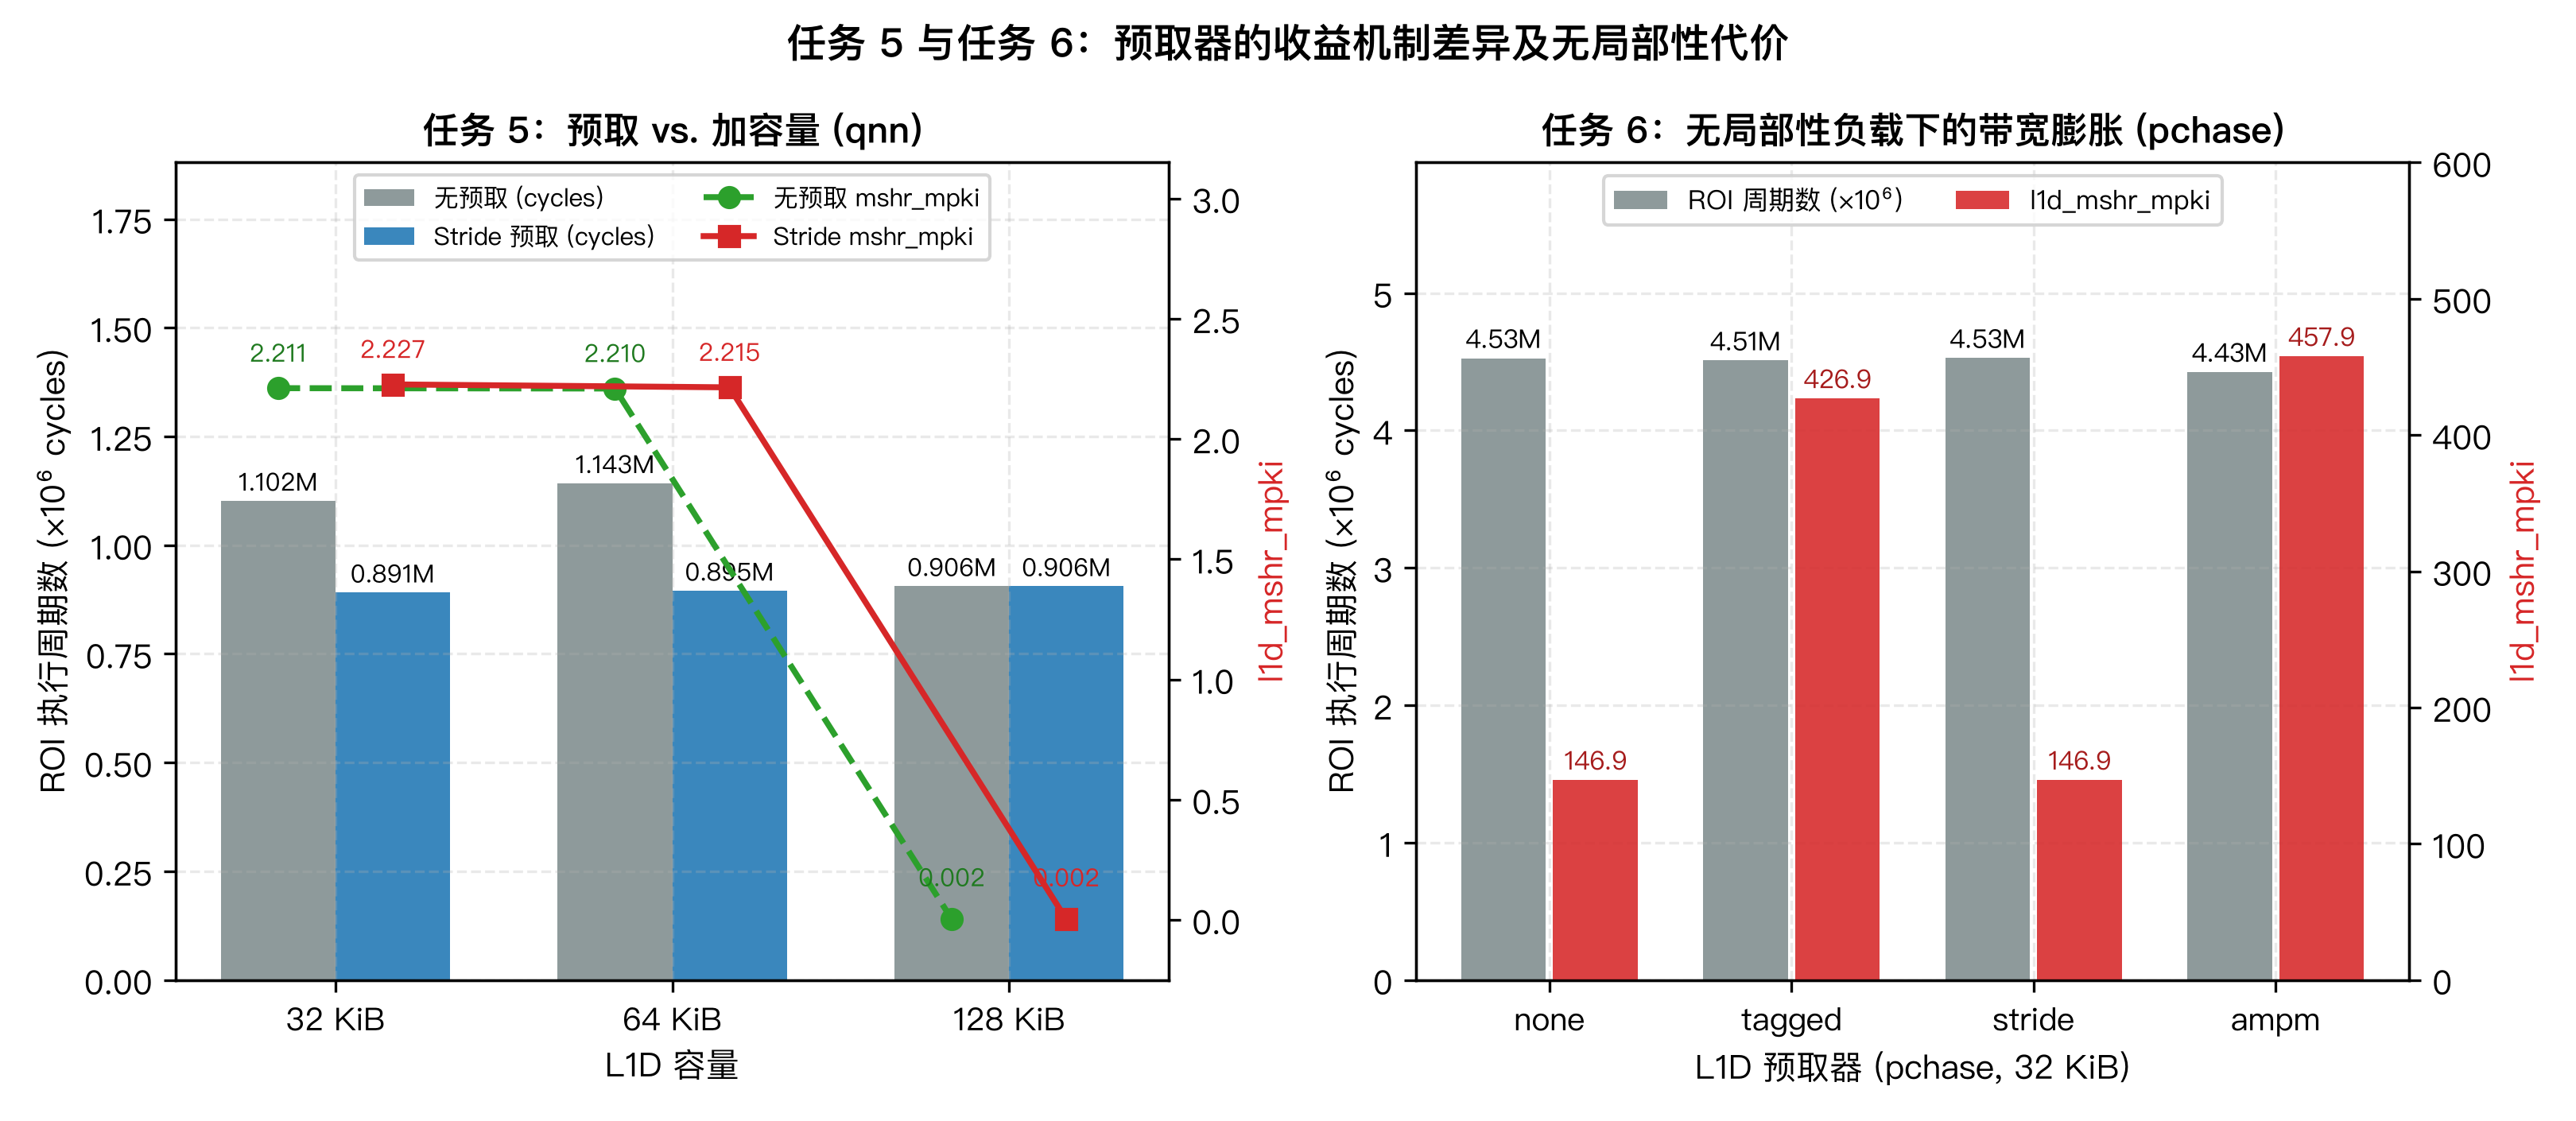
\includegraphics[width=0.98\textwidth]{fig5_pf_vs_size_pchase.png}
\caption{任务 5 与任务 6：预取与加容量的流量分化及 \texttt{pchase} 下的预取带宽膨胀}
\label{fig:pf_vs_size_pchase}
\end{figure}

\begin{enumerate}
  \item \textbf{性能与流量的极端背离（问题 1）：}\texttt{tagged} 性能几乎不变（仅快 0.38\%），\texttt{l1d\_mshr\_mpki} 却飙升至 $426.922$（暴涨 \textbf{2.91 倍}）；\texttt{ampm} 仅快 2.21\%（源自准确率 3.88\% 偶发命中的邻近节点），流量却高达 $457.909$（暴涨 \textbf{3.12 倍}，发出 42.5 万次盲目预取且 96.1\% 全部作废）；唯有自带置信度计数器的 \texttt{stride} 在发现相邻地址步长不稳后停止发射（全 ROI 仅发 4 次），保住了 $1.00\times$ 原始流量。
  \item \textbf{“性能不变、流量涨到 3 倍”在三类场景下的不可接受性（问题 2）：}
  \begin{itemize}
    \item \textbf{手机/移动端 SoC：}受电池容量与无风扇散热包络（TDP 仅数瓦）限制，3 倍片上/片外总线翻涌会带来数倍无效 SRAM Tag 查询与内存队列功耗，急剧缩短续航并触发热节流降频。
    \item \textbf{数据中心服务器：}集群总体拥有成本（TCO）高度受限于电费与散热上限，在无收益负载上白耗 3 倍带宽等于直接压低“每瓦性能（Perf/Watt）”与机柜计算密度。
    \item \textbf{多核共享带宽系统：}共享 L2 端口、片上互联（NoC）与 DRAM 通道是所有核心争用的稀缺资源；单一低局部性线程制造的 3 倍垃圾预取流量会造成队列拥塞（Queueing Delay），把同片延迟敏感服务（如 RPC、数据库查询）的尾延迟拉高数倍。
  \end{itemize}
  \item \textbf{硬件动态关闭判据设计（问题 3）：}应使用任务 4 与任务 6 中见证过的\textbf{预取准确率 \texttt{l1d\_pf\_accuracy}（即滑窗期内的 $\mathrm{pfUseful}/\mathrm{pfIssued}$）}作为核心关闭/降档判据（注意不可用 \texttt{l1d\_pf\_coverage} 单独判定，因 \texttt{ampm} 在无用场景也能“碰巧”覆盖 8.6\% 却伴随 3.88\% 的灾难级准确率）。具体工程方案：以每 $N$ 次预取发射或每 $T$ 周期为一个评估窗口（Epoch），在主硬件中引入双阈值迟滞状态机——当窗口准确率持续低于 $15\%$（如 \texttt{pchase} 下仅 $3.9\%$--$4.2\%$）时逐步降低预取度（\texttt{degree}: $4 \to 1$）直至关闭预取输出；同时保留极低开销的“影子训练表”（只学习不实际下发总线请求，或每 16 个窗口以 \texttt{degree=1} 试探 16 次），一旦工作阶段切换回规则流且影子准确率回升至 $30\%$ 以上，即刻重新使能预取器。
\end{enumerate}

\section{思考题}

\subsection*{思考题 1：LRU 的隐含前提与最好/最差访问模式}
\addcontentsline{toc}{subsection}{思考题 1：LRU 的隐含前提与最好/最差访问模式}
本次实验 \texttt{lru} 命中率为精确的 0，说明“LRU 是好策略”省略了一个关键前提：\textbf{被测工作集或热数据子集必须满足“最近访问过的块近期大概率再次使用”的时间局部性假设，且循环周期内的活跃工作集尺寸不能大于 Cache 容量 $C$}。
\begin{itemize}
  \item \textbf{让 LRU 表现最好的访问模式：}存在强时间局部性且包含一次性流干扰的偏斜热点模式——例如工作集 $\le C$ 的重复内核访问，或“少数高频热块反复读写 $+$ 少量一次性偶发访问”混合流（热块因持续被访问而保持最新时间戳，偶发冷块自然沉底淘汰，LRU 逼近 OPT）。
  \item \textbf{让 LRU 表现最差的访问模式：}工作集恰好略大于 Cache 容量（$W > C$，如本实验 98 KiB $> 64$ KiB）的\textbf{周期性顺序循环扫描}（$b_1, b_2, \dots, b_N, b_1, b_2, \dots$ 且 $N > A$），每次需要用到的块恰好是刚被 LRU 淘汰掉的最老块，命中率严格归零。
\end{itemize}

\subsection*{思考题 2：Random 替换策略是否被低估了？}
\addcontentsline{toc}{subsection}{思考题 2：Random 替换策略是否被低估了？}
在任务 1 中 \texttt{random} 以零状态位打败了 LRU、FIFO、TreePLRU 以及全部 8 个论文策略，确实在许多场景下被低估，需从三方面辩证评估：
\begin{itemize}
  \item \textbf{硬件代价：}极低——不需要每行维护 LRU 年龄位/时间戳或比较树（\texttt{area.py} 中记为 0 状态位），只需一个廉价的全局 LFSR 伪随机生成器，面积、连线电容与命中路径功耗接近于零。
  \item \textbf{可预测性：}较差——同次运行受随机种子与偶发冲突扰动存在性能波动（如任务 1c 中在正常 128 KiB 负载下因随机误踢仍产生了 $126$ 次失效，比 LRU 的 $14$ 次慢 $0.45\%$），也不利于实时系统的最坏执行时间（WCET）静态分析。
  \item \textbf{最坏情况保证：}极佳（抗病态鲁棒性强）——确定性策略（LRU/FIFO）针对特定周期序列存在 0\% 命中率的确定性最坏输入，而 Random 通过随机化打破了固定淘汰序与访问周期的相位锁定，从而保证只要每组有 $A$ 路、扫描 $N$ 块，均摊命中率不会跌至 0，拥有良好的最坏情况期望下界（$A/N$ 级别，实测拿到了 OPT 收益的 48.9\%）。因此 ARM Cortex-R/A 等注重能效的早期或中端核常采用 Pseudo-Random 替换。
\end{itemize}

\subsection*{思考题 3：适用于任意一级 Cache 的单一可测量判据}
\addcontentsline{toc}{subsection}{思考题 3：适用于任意一级 Cache 的单一可测量判据}
将任务 3 结论改写为仅依赖单一可测量指标 \texttt{refsPerInsertion}（每装入一个块平均经历的 \texttt{touch()} 次数）的通用事先判据：
\begin{quote}
\textbf{“插入位置型替换策略是否有效的判据取决于该级 Cache 的 \texttt{refsPerInsertion}：只有当 $\text{refsPerInsertion} \lesssim 1\text{--}2$（块装入后在同轮次内基本不发生连续复用，如任务 3c 中 L2 的 $0.62$）时，插入位置优先级才不被立刻抹除、策略方能生效；而当 $\text{refsPerInsertion} \gg 1$（如任务 3b 中 L1D 的 $112.27$）时，大量块内或短期命中会瞬间覆写插入位置，必须依赖牺牲者选择型策略（或把插入赌注改为累积制计数）。”}
\end{quote}

\subsection*{思考题 4：运行时可配置的代价与现代处理器实例}
\addcontentsline{toc}{subsection}{思考题 4：运行时可配置的代价与现代处理器实例}
在真实芯片中将设计参数做成运行时可配置的代价涵盖四方面：（1）控制寄存器（CSR/MSR）与配置解码状态机面积；（2）数据/控制路径上的多路选择器（MUX）、三态旁路及由此拉长的关键路径时序裕量（甚至降低最高主频）；（3）多种模式下的动态功耗泄漏；以及（4）指数级膨胀的流片前形式验证与功耗/时序签核（Sign-off）空间。

现代处理器中真实做成了运行时可配置的 Cache 参数实例：
\begin{enumerate}
  \item \textbf{硬件预取器开关配置寄存器（如 Intel MSR \texttt{0x1A4} \texttt{MISC\_FEATURE\_CONTROL}）：}允许 BIOS/OS 在运行时逐位独立开启或关闭 L2 Hardware Prefetcher、Adjacent Cache Line Prefetcher、DCU Streamer 与 DCU IP Prefetcher，用于在随机内存型数据库或延迟敏感多核任务中抑制预取带宽污染。
  \item \textbf{Cache 路划分与容量配额（如 Intel CAT 的 \texttt{IA32\_L3\_MASK\_n} / ARM MPAM）：}通过写配置寄存器为不同核或容器指定可用 LLC Way 的掩码（Way-bitmask），在运行时动态重配置各任务可见的相联度与容量上限；此外还有 NVIDIA GPU（如 Volta/Ampere/Hopper SM）允许运行时在统一 128--256 KiB SRAM 中动态切分 L1 数据 Cache 与 Shared Memory 的容量配比。
\end{enumerate}

\subsection*{思考题 5：对实验二 AMAT 模型的复盘}
\addcontentsline{toc}{subsection}{思考题 5：对实验二 AMAT 模型的复盘}
实验二以 AMAT（$\mathrm{AMAT} = T_{\text{hit}} + \text{MissRate} \times T_{\text{miss}}$）指导容量选择，本次实验至少有两组实测数据直接暴露了传统单机静态 AMAT 模型的盲区：
\begin{enumerate}
  \item \textbf{“失效率剧变但性能几乎不变”（任务 6）：}在 \texttt{pchase} 上开启 \texttt{ampm} 预取后，下级请求强度（\texttt{l1d\_mshr\_mpki}）从 $146.93$ 暴涨至 $457.91$（$3.12\times$），而周期数仅变化 $-2.21\%$；若在任务 4 的 \texttt{qnn} 上对比 \texttt{none} 与 \texttt{tagged/stride/ampm}，表观需求失效率从 $12.32\%$ 骤降到 $0.21\%$--$0.22\%$，若按 AMAT 公式会以为仅能靠降低的失效率获得加速——但实际真实带宽流量 \texttt{l1d\_mshr\_mpki} 完全不变（$2.21 \to 2.22$），加速完全来自预取对缺失延迟的提前重叠，一旦带宽饱和（多核竞争），AMAT 的固定常数 $T_{\text{miss}}$ 立即崩溃。
  \item \textbf{“真实流量不变但性能大变”（任务 4）及“失效率小幅上升但整机性能不变”（任务 1a/3a）：}在任务 4 中，\texttt{none} 与 \texttt{tagged/stride} 的 \texttt{l1d\_mshr\_mpki} 同为 $2.21$--$2.23$（下行流量几乎一模一样），执行周期却从 $1\,102\,090$ 大幅下降 $19.2\%$ 至 $890\,858$！原因在于 AMAT 假设每次 Miss 串行付出全部 $T_{\text{miss}}$，完全无法刻画乱序核的 MLP 并行重叠以及硬件预取器把“临界路径阻塞延迟”转化为“后台异步预取时间”的隐藏能力。
\end{enumerate}

\subsection*{思考题 6：贯穿题——将 CPU 从 \texttt{o3} 换成 \texttt{timing} 后任务 1 排名的变化预测}
\addcontentsline{toc}{subsection}{思考题 6：贯穿题——将 CPU 从 \texttt{o3} 换成 \texttt{timing} 后任务 1 排名的变化预测}
\textbf{预测（待实验四验证）：}若把 CPU 模型从乱序非阻塞的 \texttt{o3} 换成单发射顺序阻塞式访存的 \texttt{timing}，\textbf{任务 1（64 KiB / 4 路 L1D）各替换策略的性能相对排名基本保持不变（\texttt{lfu} 仍最优、\texttt{mru} 次之、\texttt{random} 第三，\texttt{lru} 与 8 个插入位置策略仍垫底且无效），但有效策略相对于 \texttt{lru} 的绝对周期加速幅度将会显著扩大}。理由有两点：
\begin{enumerate}
  \item 决定 L1D 命中与否的是 \texttt{dot\_i8()} 逐字节线性访存地址流与工作集大小（98 KiB $> 64$ KiB），\texttt{timing} 下每块仍会产生数十次块内顺序命中（\texttt{refsPerInsertion} 依然很大，继续抹除 \texttt{lip/bip/rrip} 的插入位置），而 \texttt{lfu/mru/random} 仍能钉住部分热块，因此\textbf{失效数与策略优劣顺序不会翻转}（在实验四无阻塞合并的微调下甚至更贴近理论 $(A-1)/N$）；
  \item 然而在 \texttt{o3} 下，高内存级并行（\texttt{l1d\_mlp} $\approx 15.8$）与长乱序窗口把大量 L2 缺失延迟互相重叠隐藏了，使 $-45.8\%$ 的 MSHR 失效降幅在 \texttt{o3} 上只转化为 $-9.38\%$ 的周期收益；换成一次仅能挂起 1 个阻塞访存的 \texttt{timing} 后，每一次 L1D MSHR 缺失都直接按串行全额停顿 CPU，失效数的下降将近似线性地转化为更大的总周期缩减（预期加速比将远超 $9.38\%$）。
\end{enumerate}

\section{实验总结}
本次实验首次完成了修改 gem5 C++ 内核、注册 \texttt{SimObject} 并增量重编译的完整系统工程训练，并基于 \texttt{qnn} 与 \texttt{pchase} 揭示了存储层次控制逻辑的四条深刻规律：
\begin{enumerate}
  \item \textbf{替换策略依赖访问模式与位置层级：}在循环扫描下精确 LRU 命中率归零且与相联度无关；但脱离病态后 MRU 反成最差，实验必须配备无病态对照组。
  \item \textbf{源码修改须先验证后扩展：}哪怕仅改动 \texttt{getVictim()} 的一个比较符，忽略空路 \texttt{lastTouchTick == 0} 保护也会令 4 路 Cache 退化；坚持“先逐位对齐、再参数化、再加统计”是排查模拟器错误的关键工程习惯。
  \item \textbf{\texttt{refsPerInsertion} 决定策略生效边界：}L1D 上 $112.27$ 次/块的连续复用在 $17.25$ 周期内抹除了全部 8 种插入位置策略的优先级；到了 \texttt{refsPerInsertion} 仅 $0.62$ 的 L2，这些策略随即爆发 $34.6\%$--$43.1\%$ 的威力。
  \item \textbf{预取器用流量换时间，不可替代容量：}在单核面积受限场景下 \texttt{32kB + stride} 能以不足 1/3 的 L1D 面积跑赢 \texttt{128kB}，但它未能消灭 L2 下行流量且在无局部性负载上存在带宽膨胀风险，必须结合准确率和多核共享约束权衡取舍。
\end{enumerate}

\clearpage
\appendix
\section*{附录：实验源代码与核心运行脚本}
\addcontentsline{toc}{section}{附录：实验源代码与核心运行脚本}

\subsection*{A.1 \texttt{gem5/src/mem/cache/replacement\_policies/cssys\_rp.hh}}
\begin{lstlisting}[language=C++,caption={最终版 cssys\_rp.hh 完整源码}]
/**
 * @file
 * Declaration of the Cssys replacement policy supporting configurable
 * LRU/MRU victim selection and insertion/reuse instrumentation statistics.
 */

#ifndef __MEM_CACHE_REPLACEMENT_POLICIES_CSSYS_RP_HH__
#define __MEM_CACHE_REPLACEMENT_POLICIES_CSSYS_RP_HH__

#include <cstdint>

#include "base/statistics.hh"
#include "base/stats/group.hh"
#include "base/types.hh"
#include "mem/cache/replacement_policies/base.hh"

namespace gem5
{

struct CssysRPParams;

namespace replacement_policy
{

class Cssys : public Base
{
  protected:
    /** Per-line replacement metadata for policy order and reuse tracking. */
    struct CssysReplData : ReplacementData
    {
        /** Tick on which the entry was last accessed (0 means invalid/empty). */
        Tick lastTouchTick;
        /** Tick on which the entry was inserted via reset(). */
        Tick insertTick;
        /** Number of demand/hit touches since insertion. */
        uint64_t refCount;

        CssysReplData() : lastTouchTick(0), insertTick(0), refCount(0) {}
    };

    /** Runtime policy switch: false = LRU (<), true = MRU (>). */
    const bool evictMru;

    /**
     * Instrumentation statistics group. Declared mutable because the Base
     * replacement interface declares touch(), reset(), and getVictim() const.
     */
    struct CssysStats : public statistics::Group
    {
        CssysStats(statistics::Group *parent);

        statistics::Scalar insertions;
        statistics::Scalar touches;
        statistics::Scalar victimizations;
        statistics::Scalar deadOnArrival;
        statistics::Scalar victimRefSum;
        statistics::Scalar firstTouchDelaySum;
        statistics::Scalar firstTouchCount;

        statistics::Formula refsPerInsertion;
        statistics::Formula deadFraction;
        statistics::Formula avgFirstTouchDelay;
    };
    mutable CssysStats cssysStats;

  public:
    typedef CssysRPParams Params;
    Cssys(const Params &p);
    ~Cssys() = default;

    void invalidate(const std::shared_ptr<ReplacementData>& replacement_data)
                                                                    override;
    void touch(const std::shared_ptr<ReplacementData>& replacement_data) const
                                                                     override;
    void reset(const std::shared_ptr<ReplacementData>& replacement_data) const
                                                                     override;
    ReplaceableEntry* getVictim(const ReplacementCandidates& candidates) const
                                                                     override;
    std::shared_ptr<ReplacementData> instantiateEntry() override;
};

} // namespace replacement_policy
} // namespace gem5

#endif // __MEM_CACHE_REPLACEMENT_POLICIES_CSSYS_RP_HH__
\end{lstlisting}

\subsection*{A.2 \texttt{gem5/src/mem/cache/replacement\_policies/cssys\_rp.cc}}
\begin{lstlisting}[language=C++,caption={最终版 cssys\_rp.cc 完整源码}]
/**
 * @file
 * Implementation of the Cssys replacement policy with evict_mru switching
 * and insertion/reuse instrumentation statistics.
 */

#include "mem/cache/replacement_policies/cssys_rp.hh"

#include <cassert>
#include <memory>

#include "params/CssysRP.hh"
#include "sim/cur_tick.hh"

namespace gem5
{

namespace replacement_policy
{

Cssys::Cssys(const Params &p)
  : Base(p), evictMru(p.evict_mru), cssysStats(this)
{
}

Cssys::CssysStats::CssysStats(statistics::Group *parent)
  : statistics::Group(parent),
    ADD_STAT(insertions, statistics::units::Count::get(),
             "Number of block insertions (reset calls)"),
    ADD_STAT(touches, statistics::units::Count::get(),
             "Number of cache hit updates (touch calls)"),
    ADD_STAT(victimizations, statistics::units::Count::get(),
             "Number of valid victims evicted"),
    ADD_STAT(deadOnArrival, statistics::units::Count::get(),
             "Number of victims evicted with zero hits after insertion"),
    ADD_STAT(victimRefSum, statistics::units::Count::get(),
             "Total touches accumulated by evicted victims"),
    ADD_STAT(firstTouchDelaySum, statistics::units::Tick::get(),
             "Sum of ticks from insertion to first hit"),
    ADD_STAT(firstTouchCount, statistics::units::Count::get(),
             "Number of blocks experiencing at least one hit"),
    ADD_STAT(refsPerInsertion, statistics::units::Rate<
             statistics::units::Count, statistics::units::Count>::get(),
             "Average touches per block insertion"),
    ADD_STAT(deadFraction, statistics::units::Ratio::get(),
             "Fraction of victims evicted without any hit"),
    ADD_STAT(avgFirstTouchDelay, statistics::units::Tick::get(),
             "Average ticks between insertion and first hit")
{
    refsPerInsertion = touches / insertions;
    deadFraction = deadOnArrival / victimizations;
    avgFirstTouchDelay = firstTouchDelaySum / firstTouchCount;
}

void
Cssys::invalidate(const std::shared_ptr<ReplacementData>& replacement_data)
{
    auto d = std::static_pointer_cast<CssysReplData>(replacement_data);
    d->lastTouchTick = Tick(0);
    d->insertTick = Tick(0);
    d->refCount = 0;
}

void
Cssys::touch(const std::shared_ptr<ReplacementData>& replacement_data) const
{
    auto d = std::static_pointer_cast<CssysReplData>(replacement_data);

    if (d->refCount == 0) {
        cssysStats.firstTouchDelaySum += curTick() - d->insertTick;
        cssysStats.firstTouchCount++;
    }
    d->refCount++;
    d->lastTouchTick = curTick();
    cssysStats.touches++;
}

void
Cssys::reset(const std::shared_ptr<ReplacementData>& replacement_data) const
{
    auto d = std::static_pointer_cast<CssysReplData>(replacement_data);
    d->lastTouchTick = curTick();
    d->insertTick = curTick();
    d->refCount = 0;
    cssysStats.insertions++;
}

ReplaceableEntry*
Cssys::getVictim(const ReplacementCandidates& candidates) const
{
    assert(candidates.size() > 0);

    ReplaceableEntry* victim = candidates[0];
    for (const auto& candidate : candidates) {
        auto cand_data = std::static_pointer_cast<CssysReplData>(
            candidate->replacementData);

        if (cand_data->lastTouchTick == 0) {
            victim = candidate;
            break;
        }

        Tick victim_tick = std::static_pointer_cast<CssysReplData>(
            victim->replacementData)->lastTouchTick;
        bool better = evictMru ? (cand_data->lastTouchTick > victim_tick)
                               : (cand_data->lastTouchTick < victim_tick);
        if (better) {
            victim = candidate;
        }
    }

    auto victim_data = std::static_pointer_cast<CssysReplData>(
        victim->replacementData);
    if (victim_data->lastTouchTick != 0) {
        cssysStats.victimizations++;
        cssysStats.victimRefSum += victim_data->refCount;
        if (victim_data->refCount == 0) {
            cssysStats.deadOnArrival++;
        }
    }

    return victim;
}

std::shared_ptr<ReplacementData>
Cssys::instantiateEntry()
{
    return std::shared_ptr<ReplacementData>(new CssysReplData());
}

} // namespace replacement_policy
} // namespace gem5
\end{lstlisting}

\subsection*{A.3 自动化实验脚本 \texttt{lab-3/run.sh}}
\begin{lstlisting}[language=bash,caption={实验三全套实验与报告生成脚本（run.sh）}]
#!/usr/bin/env bash
set -euo pipefail

cd "$(dirname "$0")"
CSSYS_SETUP_FOR_BUILD=1 source ../setup.sh

# Task 1a: L1D replacement policies (64 KiB / 4-way cyclic scan pathology)
python3 framework/sweep.py --name lab3_repl --bench qnn --bench-args "8 2799" \
  --base "--cpu o3 --l1d-size 64kB --l1d-assoc 4" \
  --vary l1d-repl=lru,fifo,secondchance,treeplru,lfu,random,mru,lip,bip,rrip,brrip,nru,drrip,ship,ship_pc \
  --jobs 8
python3 framework/report.py results/lab3_repl.csv cycles ipc l1d_misses l1d_mshr_misses l1d_mshr_mpki > results/lab3_repl_report.txt

grep -A3 'replacement_policy' out/sweeps/lab3_repl/p007_l1d-repl-lip/config.ini > results/task3_config_check.txt
grep -A6 'replacement_policy' out/sweeps/lab3_repl/p010_l1d-repl-brrip/config.ini >> results/task3_config_check.txt

# Task 1b: Associativity self-check (64 KiB, 2/4/8/16 ways)
python3 framework/sweep.py --name lab3_assoc --bench qnn --bench-args "8 2799" \
  --base "--cpu o3 --l1d-size 64kB" \
  --vary l1d-assoc=2,4,8,16 --vary l1d-repl=lru,mru --jobs 8
python3 framework/report.py results/lab3_assoc.csv cycles ipc l1d_mshr_misses l1d_mshr_mpki > results/lab3_assoc_report.txt

# Task 1c: Control group without pathology (128 KiB / 4-way)
python3 framework/sweep.py --name lab3_nopath --bench qnn --bench-args "8 2799" \
  --base "--cpu o3 --l1d-size 128kB --l1d-assoc 4" \
  --vary l1d-repl=lru,random,mru,bip --jobs 4
python3 framework/report.py results/lab3_nopath.csv cycles ipc l1d_mshr_misses l1d_mshr_mpki > results/lab3_nopath_report.txt

# Task 2c & 3b: Four-way verification & L1D CssysStats instrumentation
python3 framework/sweep.py --name lab3_mine3 --bench qnn --bench-args "8 2799" \
  --base "--cpu o3 --l1d-size 64kB --l1d-assoc 4" \
  --vary l1d-repl=lru,cssys,mru,cssys_mru --jobs 4
python3 framework/report.py results/lab3_mine3.csv cycles ipc l1d_misses l1d_mshr_misses l1d_mshr_mpki > results/lab3_mine3_report.txt

python3 framework/sweep.py --name lab3_mine4 --bench qnn --bench-args "8 2799" \
  --base "--cpu o3 --l1d-size 64kB --l1d-assoc 4" \
  --vary l1d-repl=cssys --jobs 1

# Task 3c: L2 replacement policies (64 KiB / 4-way L2) + CssysStats
python3 framework/sweep.py --name lab3_l2repl --bench qnn --bench-args "8 2799" \
  --base "--cpu o3 --l2-size 64kB --l2-assoc 4" \
  --vary l2-repl=lru,fifo,secondchance,treeplru,lfu,random,mru,lip,bip,rrip,brrip,nru,drrip,ship,ship_pc \
  --jobs 8
python3 framework/report.py results/lab3_l2repl.csv cycles ipc l2_accesses l2_mshr_misses l2_mshr_mpki > results/lab3_l2repl_report.txt

python3 framework/sweep.py --name lab3_l2cssys --bench qnn --bench-args "8 2799" \
  --base "--cpu o3 --l2-size 64kB --l2-assoc 4" \
  --vary l2-repl=cssys --jobs 1

# Task 4-6: Prefetcher evaluations & area/energy comparisons
python3 framework/sweep.py --name lab3_pf --bench qnn --bench-args "8 2799" \
  --base "--cpu o3" --vary l1d-pf=none,tagged,stride,bop,ampm,isb --jobs 6
python3 framework/report.py results/lab3_pf.csv cycles ipc l1d_misses l1d_mshr_mpki \
  l1d_pf_issued l1d_pf_useful l1d_pf_accuracy l1d_pf_coverage l1d_mlp > results/lab3_pf_report.txt

python3 framework/sweep.py --name lab3_pf_vs_size --bench qnn --bench-args "8 2799" \
  --base "--cpu o3" --vary l1d-size=32kB,64kB,128kB \
  --vary l1d-pf=none,stride --jobs 6
python3 framework/report.py results/lab3_pf_vs_size.csv cycles ipc l1d_misses l1d_mshr_mpki \
  l1d_pf_issued l1d_pf_useful l1d_pf_accuracy l1d_mlp > results/lab3_pf_vs_size_report.txt
python3 framework/area.py out/sweeps/lab3_pf_vs_size/*/ > results/lab3_pf_vs_size_area.txt

python3 framework/sweep.py --name lab3_pf_pchase --bench pchase \
  --bench-args "256 200000 2799" \
  --base "--cpu o3" --vary l1d-pf=none,tagged,stride,ampm --jobs 4
python3 framework/report.py results/lab3_pf_pchase.csv cycles ipc l1d_mshr_mpki \
  l1d_pf_issued l1d_pf_useful l1d_pf_accuracy dram_bytes > results/lab3_pf_pchase_report.txt
\end{lstlisting}

\end{document}
